\section{Gauge Convolutions}\label{sec:gauge_cnns}

The diversity of techniques specific to particular manifolds, examined in the previous section, raises a fundamental question: is there a unifying framework that transcends specific geometries? The answer emerges from \textbf{gauge theory}, providing general principles for the design of architectures invariant under local transformations.

Gauge convolutions represent a profound conceptual extension of the convolutional paradigm. While classical convolutions exploit global symmetries (translations), and geometric extensions exploit intrinsic symmetries of specific manifolds, \textbf{gauge convolutions} address local symmetries that may vary from point to point in space. This approach, inspired by fundamental physics, provides an elegant mathematical framework for the construction of neural networks with sophisticated invariance properties.

\subsection{From Global to Local Symmetries: Intuitive Motivation}\label{subsec:motivacion_simetrias_locales}

Before delving into the mathematical formalism, it is crucial to understand \textit{why} we need local symmetries and how they emerge naturally in real problems. This section provides the intuition and motivation necessary to justify the mathematical complexity that follows.

\begin{figure}[htbp]
	\centering
	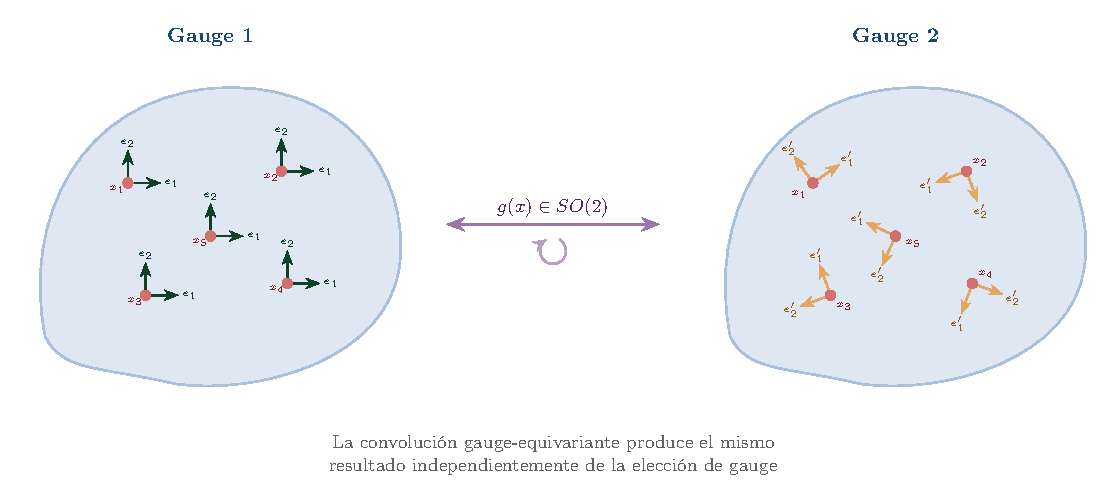
\includegraphics[width=0.90\textwidth]{images/gauge_freedom}
	\caption[Gauge freedom: choice of local frames]{Gauge freedom: the same surface admits different choices of local frames (Gauge 1 and Gauge 2). The gauge-equivariant convolution produces identical results regardless of the gauge choice, connected by pointwise transformations $g(x) \in SO(2)$.}
	\label{fig:gauge_freedom}
\end{figure}

\subsubsection{The problem of rigid symmetries}

Classical CNNs assume that the same transformations (translations) are valid throughout the domain. This assumption works well for flat images, but fails systematically when the data has intrinsic geometric structure.

\begin{example}[Rotations on a Sphere]
Consider an image of the Earth projected onto a sphere. If we apply a global rotation of $90^\circ$ around the north-south axis:
\begin{itemize}
    \item At the equator, the rotation preserves local shapes perfectly
    \item Near the poles, the same rotation causes severe distortion
    \item An image of a continent near the north pole looks completely different after the global rotation
\end{itemize}
This example illustrates that \textbf{the appropriate transformation depends on the position}.
\end{example}

\textbf{Failure of Global Equivariance.} In curved spaces or those with non-trivial topology, applying the same transformation everywhere can:
\begin{enumerate}
    \item \textbf{Break the natural geometric structure} of the domain
    \item \textbf{Introduce artificial distortions} that did not exist in the original data
    \item \textbf{Violate the physical principles} that govern the modeled phenomenon
\end{enumerate}

\subsubsection{Fundamental physical analogies}

Gauge theory has its roots in physics, where it describes phenomena in which the mathematical description depends on arbitrary choices of local coordinates or references.

\begin{example}[Electromagnetism: The Classical Paradigm]
In electromagnetism, the observable physical fields (such as the electric field $\mathbf{E}$ and magnetic field $\mathbf{B}$) do not depend on how we choose to describe the electromagnetic potential $A_\mu(x)$.

\textbf{Gauge Freedom}: We can transform $A_\mu(x) \mapsto A_\mu(x) + \partial_\mu \Lambda(x)$ where $\Lambda(x)$ is an arbitrary function that can vary from point to point.

\textbf{Physical Invariance}: The observable fields remain unaltered:
\begin{align}
\mathbf{E} &= -\nabla \phi - \frac{\partial \mathbf{A}}{\partial t} \\
\mathbf{B} &= \nabla \times \mathbf{A}
\end{align}
remain invariant under the gauge transformation.

\textbf{Connection with Deep Learning}: Just as physical laws should not depend on our choice of coordinates, neural representations should not depend on arbitrary choices of local reference systems.
\end{example}

\begin{example}[Navigation on Earth: Local Coordinate Systems]
Imagine you are developing a global navigation system:
\begin{itemize}
    \item In New York, it is natural to use coordinates that point toward ``geographic north''
    \item In Sydney, ``geographic north'' points in a completely different direction in three-dimensional space
    \item Nevertheless, the \textit{local relations} (left, right, forward, backward) are consistent in both cities
\end{itemize}

A \textbf{gauge equivariant} neural network can learn to recognize patterns that are invariant to these choices of local coordinate system, while maintaining the ability to exploit the real geometric structure of the problem.
\end{example}

\subsubsection{Conceptual progression: from simple to complex}

To build intuition, let us consider the natural progression from simple cases toward full generality:

\begin{enumerate}
    \item \textbf{Classical CNNs}: A single transformation (translation) valid globally
    \item \textbf{Group-CNNs}: A finite set of transformations valid globally
    \item \textbf{CNNs on Manifolds}: Transformations dictated by the specific geometry of the manifold
    \item \textbf{Gauge CNNs}: Complete freedom to choose local transformations, subject to consistency
\end{enumerate}

\textbf{Why not simply data augmentation?} One might ask: ``Why not simply augment the data with multiple local transformations?'' The answer is fundamental:

\begin{itemize}
    \item \textbf{Data augmentation}: Hopes to achieve invariance \textit{statistically} across multiple samples
    \item \textbf{Gauge equivariance}: Guarantees \textit{exact} invariance through the architecture
    \item \textbf{Efficiency}: Gauge equivariance achieves with a single forward pass what data augmentation requires multiple evaluations for
    \item \textbf{Consistency}: Guarantees that the network cannot learn to exploit ``accidental'' transformations that do not reflect the true structure of the problem
\end{itemize}

\subsection{Concrete Example: Gauge Equivariance in Action}\label{subsec:ejemplo_gauge_equivarianza}

To make these abstract concepts concrete, let us develop a simple but illustrative example that shows how gauge transformations work in practice.

\subsubsection{Scenario: Pattern recognition on a cylindrical surface}

Consider the problem of recognizing textures on a cylinder (such as a tree trunk). The data consist of an image ``wrapped'' around the cylinder.

\begin{example}[Local Coordinate Problem on a Cylinder]
Suppose we have a tree-bark texture photographed at different positions around the trunk:
\begin{itemize}
    \item \textbf{Position A}: Photo taken facing north
    \item \textbf{Position B}: Photo taken facing east
    \item \textbf{Position C}: Photo taken facing south
\end{itemize}

At each position, we establish local coordinates $(u,v)$ where:
\begin{itemize}
    \item $u$: ``horizontal'' direction relative to the camera orientation
    \item $v$: ``vertical'' direction (along the trunk axis)
\end{itemize}

\textbf{The problem}: The same physical bark patterns appear as completely different tensors in each local coordinate system.
\end{example}

\subsubsection{Gauge solution: coherent local transformations}

\begin{definition}[Simple Gauge Transformation]
For our cylinder, a \textbf{gauge transformation} is a function $g: S^1 \times \mathbb{R} \to SO(2)$ that assigns to each point $(\theta, z)$ of the cylinder a local rotation in the tangent plane:
\begin{equation}
g(\theta, z) = \begin{pmatrix}
\cos(\phi(\theta, z)) & -\sin(\phi(\theta, z)) \\
\sin(\phi(\theta, z)) & \cos(\phi(\theta, z))
\end{pmatrix}
\end{equation}
where $\phi(\theta, z)$ can vary smoothly over the surface.
\end{definition}

\begin{example}[Gauge Convolution on the Cylinder]\label{ex:convolucion_gauge_cilindro}
A gauge equivariant convolution in this scenario would be:
\begin{equation}
[f \star \psi]_\text{gauge}(\theta, z) = \int_{N(\theta,z)} \psi\left(g(\theta', z')^{-1} \cdot \text{connect}((\theta,z), (\theta',z'))\right) f(\theta', z') \, d\theta' dz'
\end{equation}

where:
\begin{itemize}
    \item $N(\theta,z)$ is a neighborhood of the point $(\theta,z)$
    \item $\text{connect}((\theta,z), (\theta',z'))$ describes how to ``connect'' the local coordinate systems
    \item $\psi$ is a kernel that operates in the space of ``orientation differences''
\end{itemize}

\textbf{Key property}: If we apply different choices of local orientation $g(\theta,z)$ at each point, the final result of the convolution remains invariant.
\end{example}

\subsubsection{Visualization of information transport}

\begin{figure}[htbp]
	\centering
	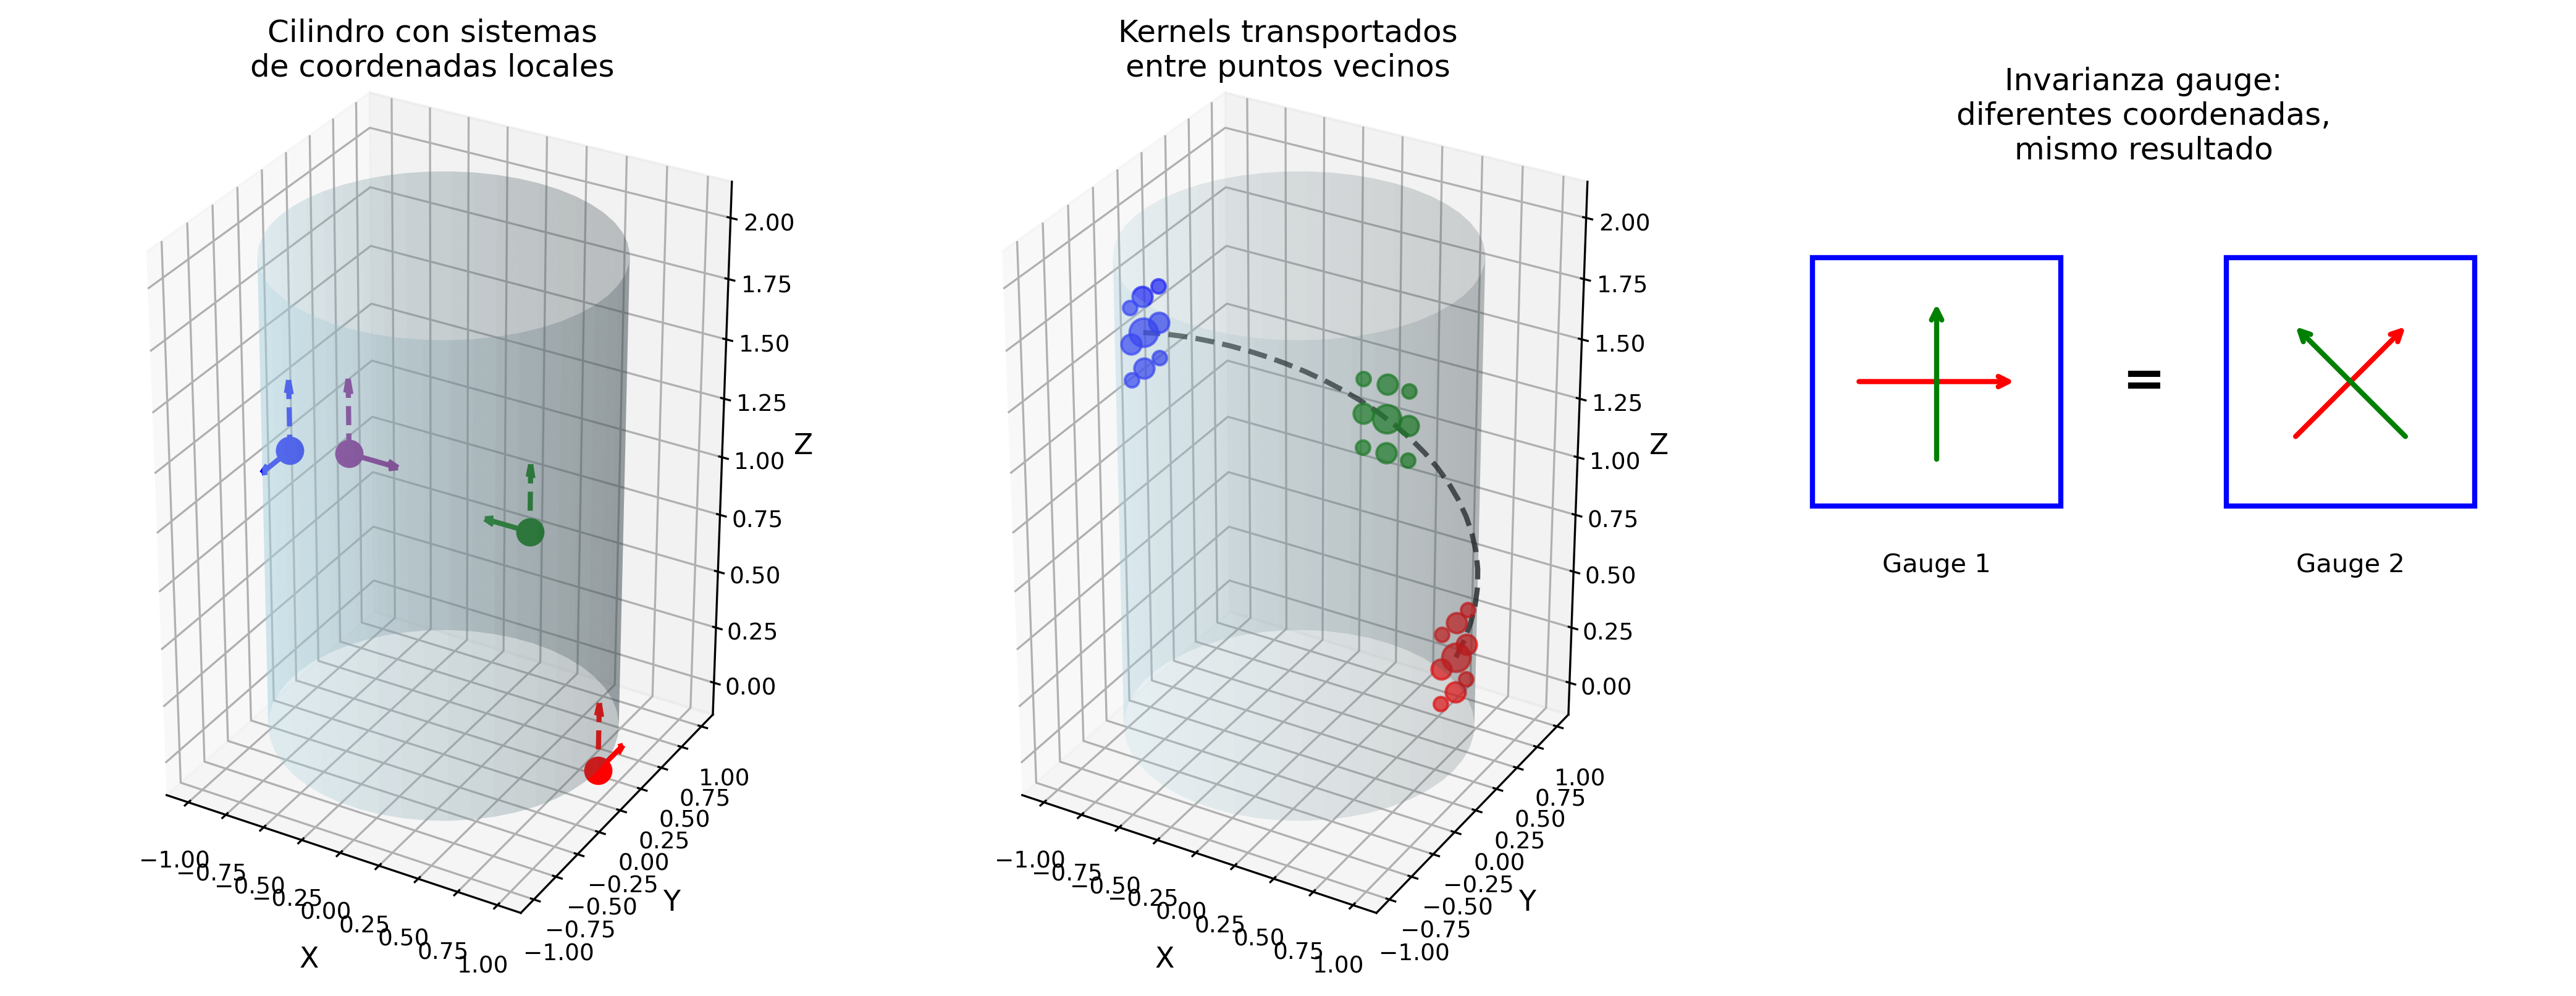
\includegraphics[width=0.95\textwidth]{images/gauge_transport_cylinder.png}
	\caption[Gauge transport on a cylinder]{Gauge transport on a cylinder. Left: local coordinate systems (tangent vectors) at different points of the cylinder. Center: convolution kernels transported along a geodesic between neighboring points. Right: the concept of gauge invariance: different choices of local orientation (Gauge 1 vs. Gauge 2) produce the same detected pattern.}
	\label{fig:gauge_transport_cylinder}
\end{figure}

\textbf{Key Intuition: Separation of Shape and Orientation.} Gauge equivariance allows the network to learn about:
\begin{itemize}
    \item \textbf{Intrinsic shape}: Which patterns are present (independent of orientation)
    \item \textbf{Spatial relations}: How patterns relate geometrically
\end{itemize}
while completely ignoring:
\begin{itemize}
    \item \textbf{Absolute orientation}: Arbitrary choices of ``north'', ``up'', etc.
    \item \textbf{Coordinate systems}: Labeling conventions that do not affect the physics
\end{itemize}

\begin{proposition}[Gauge Equivariance on the Cylinder]\label{prop:gauge_equivarianza_cilindro}
Let $f: S^1 \times \mathbb{R} \to \mathbb{R}^d$ be a feature field over the cylinder and let $g: S^1 \times \mathbb{R} \to SO(2)$ be an arbitrary gauge transformation. The gauge convolution $[f \star \psi]_{\text{gauge}}$ defined in \autoref{ex:convolucion_gauge_cilindro} satisfies:
\begin{equation}
[(\rho(g) \cdot f) \star \psi]_{\text{gauge}} = \rho(g) \cdot [f \star \psi]_{\text{gauge}}
\end{equation}
where $(\rho(g) \cdot f)(\theta, z) = g(\theta,z) \cdot f(\theta, z)$ is the pointwise gauge action.
\end{proposition}

\begin{proof}
Substituting the definition:
\begin{align}
[(\rho(g) \cdot f) \star \psi]_{\text{gauge}}(\theta, z) &= \int_{N(\theta,z)} \psi\left(g(\theta',z')^{-1} \cdot c_{(\theta,z) \to (\theta',z')}\right) g(\theta',z') f(\theta',z') \, d\theta' dz'
\end{align}
where $c_{(\theta,z) \to (\theta',z')}$ denotes the connection (parallel transport) between the local frames. Since $g(\theta',z')^{-1} g(\theta',z') = \operatorname{Id}$, the gauge transformation of the field $f$ cancels with the inverse transformation in the argument of $\psi$, leaving the result transformed by $g(\theta,z)$ at the output point.
\end{proof}

\begin{remark}[Analogy with Gauge Theories in Physics]
The mathematical structure of this proposition is identical to that of gauge theories in particle physics. In electrodynamics, the vector potential $A_\mu$ (analogous to our field $f$) transforms under a gauge change $A_\mu \to A_\mu + \partial_\mu \chi$, but the field tensor $F_{\mu\nu} = \partial_\mu A_\nu - \partial_\nu A_\mu$ (analogous to the output of the convolution) is gauge-invariant. The gauge convolution of Cohen et al. implements exactly this principle in the context of neural networks.
\end{remark}

\subsection{Mathematical Foundations of Gauge Theory}\label{subsec:fundamentos_matematicos_gauge}

The fundamental distinction between global and local symmetries is formalized as follows:

\begin{definition}[Local vs. Global Transformation]
For a group $G$ and a function $f: \mathcal{M} \to \mathbb{R}^d$:

\textbf{Global Transformation}: $T_g[f](x) = \rho(g) f(g^{-1} \cdot x)$, where $g \in G$ is the same element for all points $x \in \mathcal{M}$.

\textbf{Local (Gauge) Transformation}: $T_{g(\cdot)}[f](x) = \rho(g(x)) f(\phi_{g(x)}(x))$, where $g: \mathcal{M} \to G$ assigns to each point $x$ a transformation $g(x) \in G$.
\end{definition}

The freedom to choose independent local transformations raises a fundamental problem: how do we compare information between points with different coordinate systems? The answer comes from the theory of principal bundles (\autoref{def:fibrado_principal_formal}, \autoref{ch:gdl}), which associates to each point of the space all its possible local orientations. In our cylinder example, the bundle is $P = (S^1 \times \mathbb{R}) \times SO(2)$, where each point $(\theta, z, R) \in P$ represents a position with local orientation $R$.

\textbf{Connections} (\autoref{def:conexion_fibrado}) solve the comparison problem by specifying how to transport orientations between neighboring points in a consistent way, and \textbf{parallel transport} (\autoref{def:transporte_paralelo_formal}) allows objects in different fibers to be compared. For a complete exposition of this formalism, see \autoref{sec:gauges_invarianzas}.

\begin{proposition}[Topological Obstruction to Global Gauges]\label{prop:obstruccion_gauge_global}
Let $\mathcal{M}$ be a differentiable manifold and $P \to \mathcal{M}$ a principal bundle with structure group $G$. The bundle admits a global section (that is, a consistent choice of gauge over all of $\mathcal{M}$) if and only if $P$ is trivial ($P \cong \mathcal{M} \times G$). In particular:
\begin{enumerate}
    \item The frame bundle of $S^2$ does not admit a global section (by the hairy ball theorem).
    \item Every principal bundle over a contractible manifold is trivial.
\end{enumerate}
\end{proposition}

\begin{proof}
A global section $s: \mathcal{M} \to P$ induces the trivialization $\mathcal{M} \times G \to P$ given by $(x, g) \mapsto s(x) \cdot g$, which is a bundle isomorphism by the free and transitive action of $G$ on each fiber. Conversely, a trivialization $P \cong \mathcal{M} \times G$ provides the section $s(x) = (x, e)$.

For (1), a section of the orthonormal frame bundle $\operatorname{SO}(\mathcal{M})$ of $S^2$ is equivalent to a continuous field of orthonormal bases, which in particular implies a nowhere-vanishing tangent vector field, contradicting the hairy ball theorem (the Euler characteristic $\chi(S^2) = 2 \neq 0$).

For (2), every contractible manifold is homotopy equivalent to a point, hence every principal bundle over it is trivial (since bundles are classified by homotopy classes of maps to the classifying space $BG$).
\end{proof}

\begin{remark}[Implication for Neural Networks]
\autoref{prop:obstruccion_gauge_global} explains why gauge equivariance is \textit{necessary} (not merely convenient) for neural networks on general surfaces: on the sphere $S^2$ and on most manifolds of interest, there is no consistent global coordinate system. Any global parametrization has singularities (such as the poles in spherical coordinates). Gauge equivariance allows the network to be independent of these local choices, avoiding artifacts at the singularities.
\end{remark}

\subsubsection{Toward practical implementation}

The gap between theory (infinite-dimensional bundles with smooth connections) and practice (discrete neural networks with finite parameters) is significant. The pioneering work of Cohen et al.\ showed how to find discretizations that preserve the essential theoretical properties. The key lies in the fact that gauge equivariance imposes \textit{linear} constraints on the network weights, reducing the parameter space to an affine subspace that can be solved analytically before training.

\subsection{Gauge Equivariant CNNs: The Model of Cohen et al.}\label{subsec:modelo_cohen_gauge}

The seminal work of Cohen et al.~\citep{cohen2019gaugeequivariantconvolutional} represents the first success in translating abstract gauge theory into a practical and efficient neural architecture. Their key contribution was to show how to implement exact gauge equivariance while maintaining the basic structure of convolutions.

\subsubsection{Design philosophy: from the abstract to the concrete}

The approach of Cohen et al. follows a clear design philosophy:
\begin{enumerate}
    \item \textbf{Principle}: Identify the fundamental geometric properties that the architecture must preserve
    \item \textbf{Discretization}: Find a finite representation that captures these properties
    \item \textbf{Implementation}: Translate into operations that can be executed efficiently
    \item \textbf{Verification}: Demonstrate that the implementation respects the theoretical properties
\end{enumerate}

The concepts of curvature (\autoref{def:curvatura_formal}) and parallel transport (\autoref{def:transporte_paralelo_formal}), fundamental to the construction of gauge equivariant convolutions, are developed formally in \autoref{sec:gauges_invarianzas}. Curvature measures the ``integrability defect'' of the connection (how much parallel transport depends on the chosen path), while parallel transport provides the mechanism for comparing elements in different fibers.

\subsubsection{The specific case: icosahedral CNNs}

To make these abstract ideas concrete, Cohen et al. focus on a specific case that combines theoretical richness with computational feasibility.

\begin{example}[Why the Icosahedron?]
The choice of the icosahedron as a domain is not arbitrary:

\textbf{Geometric properties}:
\begin{itemize}
    \item \textbf{Best spherical approximation}: Among the regular polyhedra, it is the one that best approximates the sphere
    \item \textbf{Rich symmetry}: Symmetry group $I_h$ with 120 elements
    \item \textbf{Geodesic regularity}: Approximately uniform distances between vertices
    \item \textbf{Canonical triangulation}: Well-defined mesh structure
\end{itemize}

\textbf{Computational properties}:
\begin{itemize}
    \item \textbf{Manageable size}: 12 vertices, 20 faces, 30 edges
    \item \textbf{Systematic subdivision}: Refinement by geodesic subdivision
    \item \textbf{Barycentric coordinates}: Smooth interpolation on each triangular face
    \item \textbf{Efficient implementation}: Optimized data structure
\end{itemize}
\end{example}

\begin{definition}[Icosahedral Discretization]\label{def:discretizacion_icosaedrica}
The icosahedral discretization of the sphere $S^2$ is obtained by means of:

\textbf{Geometric construction}:
\begin{enumerate}
    \item \textbf{Inscribed icosahedron}: 12 vertices located on $S^2$ with maximal symmetry
    \item \textbf{Radial projection}: Each point of the sphere is assigned to the nearest vertex
    \item \textbf{Geodesic refinement}: Subdivision of edges by great circles
\end{enumerate}

\textbf{Parametrization}: Each point in $S^2$ is represented as:
\begin{equation}
p = \sum_{i=1}^{12} w_i v_i, \quad \sum_{i=1}^{12} w_i = 1, \quad w_i \geq 0
\end{equation}
where $\{v_i\}$ are the icosahedral vertices and $\{w_i\}$ are barycentric coordinates.
\end{definition}

\begin{definition}[Local Gauge Transformation]\label{def:transformacion_gauge_local}
In the icosahedral discretization, the local gauge transformations are defined as:
\begin{equation}
h: S^2 \to SO(2)
\end{equation}
where $h(p) \in SO(2)$ specifies the transformation at the point $p$.

\textbf{Regularity constraint}: To guarantee differentiability, it is required that:
\begin{equation}
\|h(p) - h(q)\| \leq C d(p,q)^\alpha
\end{equation}
for some constant $C$ and Hölder exponent $\alpha \in (0,1]$.
\end{definition}

\begin{definition}[Gauge Equivariant Function]\label{def:funcion_gauge_equivariante}
A function $f: S^2 \to \mathbb{R}^n$ is said to be gauge equivariant if for every gauge transformation $h$:
\begin{equation}
f^h(p) = \rho(h(p)^{-1}) f(p)
\end{equation}
where $\rho: SO(2) \to GL(\mathbb{R}^n)$ is a representation of the group.

\textbf{Important special cases}:
\begin{itemize}
    \item \textbf{Scalars} ($n=1$): $\rho$ trivial, $f^h = f$
    \item \textbf{Vectors} ($n=2$): $\rho$ is the standard representation of $SO(2)$
    \item \textbf{Complex fields}: Multiplication by $e^{i\theta}$ for rotation by angle $\theta$
\end{itemize}
\end{definition}

\begin{theorem}[Gauge Equivariant Convolution]\label{thm:convolucion_gauge_equivariante}
For gauge equivariant functions $f, g: S^2 \to \mathbb{R}^n$, their gauge convolution is defined as:
\begin{equation}
(f *_G g)(p) = \int_{S^2} f(q) \cdot G(q, p) \cdot g(q) \, d\sigma(q)
\end{equation}
where $G(q,p)$ is the gauge propagator that encodes the parallel transport from $q$ to $p$.

If $f$ and $g$ are gauge equivariant, then $f *_G g$ is also gauge equivariant.
\end{theorem}

\begin{proof}
Let $\rho_p$ be a gauge change at the point $p$ (a change of local basis of the tangent space), so that gauge equivariant functions transform as $f(p) \mapsto \rho_p \cdot f(p)$. The gauge propagator $G(q,p)$ encodes the parallel transport from $q$ to $p$ and transforms as $G(q,p) \mapsto \rho_p \cdot G(q,p) \cdot \rho_q^{-1}$ (since it changes from the basis at $q$ to the basis at $p$). Then:
\begin{align}
(f *_G g)(p) &\mapsto \int_{S^2} (\rho_q f(q)) \cdot (\rho_p G(q,p) \rho_q^{-1}) \cdot (\rho_q g(q)) \, d\sigma(q) \\
&= \rho_p \int_{S^2} f(q) \cdot G(q,p) \cdot g(q) \, d\sigma(q) = \rho_p \cdot (f *_G g)(p)
\end{align}
where we used that $\rho_q^{-1} \rho_q = \operatorname{Id}$. Thus, $f *_G g$ transforms as $\rho_p \cdot (f *_G g)(p)$, which is the gauge equivariant transformation law.
\end{proof}

\textbf{Implementation of the gauge propagator}: In practice, $G(q,p)$ is implemented by means of:

\begin{algorithm}[H]
\caption{Computation of the Icosahedral Gauge Propagator}
\begin{algorithmic}[1]
    \State \textbf{Input:} Points $q, p \in S^2$, gauge connection $\omega$
    \State Find geodesic path $\gamma: q \to p$ in the discretization
    \State Initialize group element $g = I \in SO(2)$
    \For{each edge $e$ in the path $\gamma$}
        \State Update: $g \leftarrow g \cdot \exp(-\omega_e)$
    \EndFor
    \State \textbf{Output:} $G(q,p) = g$
\end{algorithmic}
\end{algorithm}

\subsubsection{Simplified theoretical construction}

\begin{theorem}[Simplified Construction of Gauge CNNs]
To make the ideas more accessible, we present a simplified construction that retains the essential elements:

\textbf{Input data}: A function $f: V \to \mathbb{R}^d$ defined on the icosahedral vertices $V = \{v_1, \ldots, v_{12}\}$.

\textbf{Local gauge convolution}: At each vertex $v_i$:
\begin{equation}
(f * \psi)(v_i) = \sum_{j \in \mathcal{N}(i)} \psi_{ij} \cdot \Gamma_{ij} \cdot f(v_j)
\end{equation}
where:
\begin{itemize}
    \item $\mathcal{N}(i)$ are the neighboring vertices of $v_i$
    \item $\psi_{ij}$ are learnable kernel weights
    \item $\Gamma_{ij} \in SO(2)$ is the gauge transport from $v_j$ to $v_i$
\end{itemize}

\textbf{Learning the connection}: The transport elements $\Gamma_{ij}$ are parametrized as:
\begin{equation}
\Gamma_{ij} = \exp(i\theta_{ij}), \quad \theta_{ij} \in [0, 2\pi)
\end{equation}
and the angles $\{\theta_{ij}\}$ are learnable parameters of the network.

\textbf{Gauge regularization}: To avoid degenerate solutions, a regularization term is added:
\begin{equation}
\mathcal{R}(\theta) = \sum_{\text{triangles } T} \left|\sum_{(i,j) \in \partial T} \theta_{ij}\right|^2
\end{equation}
which penalizes excessive curvature (non-trivial holonomy in small triangles). This regularization is a practical consequence of the Bianchi identity~\eqref{eq:bianchi}.
\end{theorem}

\subsection{General Framework of Principal Bundles}

Beyond the icosahedral example, gauge theory provides a general framework for the design of equivariant neural architectures in complex geometric contexts.

\subsubsection{Classification of gauge structures}

Different problems require different choices of principal bundle, determined by the intrinsic symmetries of the data.

\begin{theorem}[Classification of Bundles for Deep Learning]
Let $\mathcal{M}$ be a manifold that models the data domain and $G$ the relevant symmetry group. The principal bundles appropriate for gauge equivariant architectures are classified according to:

\begin{enumerate}
\item \textbf{Trivial bundles}: $P = \mathcal{M} \times G$ when the symmetries are globally consistent
\item \textbf{Frame bundles}: When invariance under local coordinate changes is required
\item \textbf{Spin bundles}: For data with orientation structure (common in particle physics)
\item \textbf{Gauge bundles}: For fields with internal symmetries (electromagnetism, Yang-Mills fields)
\end{enumerate}
\end{theorem}

\subsubsection{Universal approximation properties}

The rigorous formulation of gauge equivariant convolutions uses parallel transport (\autoref{def:transporte_paralelo_formal}) to compare fibers at different points of the base manifold, preserving the gauge structure.

A fundamental theoretical result establishes that gauge equivariant networks possess universal approximation properties in appropriate contexts.

\begin{theorem}[Universal Gauge Approximation]
Let $\mathcal{F}_{\text{gauge}}$ be the space of functions implementable by gauge equivariant networks with sufficient depth and width. Then:

\begin{enumerate}
\item $\mathcal{F}_{\text{gauge}}$ is dense in $L^2_{\text{gauge}}(P)$, the space of square-integrable gauge equivariant functions
\item The approximation rate is $O(n^{-2/(d_{\mathcal{M}} + d_G)})$ where $d_{\mathcal{M}}$ is the dimension of the base manifold and $d_G$ the dimension of the gauge group
\item The approximation constants depend only on the curvature of the bundle and the regularity properties of the connection
\end{enumerate}

See Section~\ref{sec:aproximacion_universal_gauge} of \autoref{ch:teoremas_complementarios} for the proof sketch.
\end{theorem}

\subsection{Deeper Mathematical Foundations}

The mathematical foundations of gauge theory (including the curvature of the connection (\autoref{def:curvatura_formal}), the Cartan structure equation (\autoref{thm:cartan_estructura}) and holonomy (\autoref{def:holonomia})) are developed formally in \autoref{sec:gauges_invarianzas} of \autoref{ch:gdl}. Here we focus on the applications of these concepts to geometry and physics.

\subsubsection{Mathematical applications in geometry and physics}

The theory of gauge convolutions provides unifying frameworks for modeling phenomena where local symmetries play a fundamental role.

\paragraph{Gauge field theories}
The fundamental gauge fields of theoretical physics are naturally modeled by principal bundles with specific structure groups.

\begin{example}[Quantum Electrodynamics]
Electromagnetism is described by the principal bundle $(P, \mathcal{M}, \pi, U(1))$ where:
\begin{itemize}
\item The base manifold $\mathcal{M}$ represents spacetime
\item The group $U(1)$ encodes the electromagnetic phase transformations
\item The connection $A$ is the electromagnetic vector potential
\item The curvature $F = dA$ is the electromagnetic field tensor
\end{itemize}
\end{example}

\paragraph{Differential geometry}
Gauge structures appear naturally in the study of Riemannian manifolds and their generalizations.

\begin{example}[Orthogonal Frame Bundle]
For a Riemannian manifold $(\mathcal{M}, g)$, the orthonormal frame bundle $O(\mathcal{M})$ is a principal bundle with structure group $O(n)$. Gauge convolutions in this context respect the local isometries of the Riemannian metric.
\end{example}

\paragraph{Algebraic topology}
The characteristic classes of principal bundles provide topological invariants that completely classify gauge structures up to isomorphism.

\begin{example}[Chern Classes]
For complex bundles, the Chern classes $c_k \in H^{2k}(\mathcal{M}, \mathbb{Z})$ provide topological obstructions to the existence of global sections and connections with prescribed curvature.
\end{example}

\subsection{Theoretical Extensions and Recent Developments}

\subsubsection{Gauge CNNs in higher dimensions}

The extensions of gauge theory to higher dimensions and more complex structures represent an active area of research.

\begin{definition}[Higher-Order Principal Bundle]
A \textbf{higher-order principal bundle} is a sequence of bundles:
\begin{equation}
G \to P_n \to P_{n-1} \to \cdots \to P_1 \to \mathcal{M}
\end{equation}
where each level introduces additional symmetries. These structures model physical systems with multiple symmetry scales.
\end{definition}

\paragraph{Applications in unified field theories}
Non-abelian gauge theories (such as quantum chromodynamics) require principal bundles with non-commutative groups:

\begin{example}[Lattice QCD]
Quantum chromodynamics on a lattice is modeled by:
\begin{itemize}
\item Base manifold: Discrete spacetime lattice
\item Gauge group: $SU(3)$ (color group)
\item Fields: Gauge connections on lattice links
\item Gauge structure: Describes the fundamental interactions between quarks and gluons
\end{itemize}
\end{example}

\subsubsection{Connection with generalized Lie algebras}

Recent developments explore the connection between gauge CNNs and more general algebraic structures.

\begin{theorem}[Representation by Lie Algebras]
Every gauge CNN can be represented by a generalized Lie algebra $\mathfrak{L}$ that acts on the feature space. The structure of $\mathfrak{L}$ completely determines the equivariance properties of the network.
\end{theorem}

This representation allows:
\begin{itemize}
\item Systematic classification of gauge structures by algebraic invariants
\item Complete characterization of equivariance properties via representation theory
\item Geometric analysis of gauge moduli spaces
\end{itemize}

\subsubsection{Quantum gauge CNNs}

An emerging frontier explores the extension of gauge principles to the domain of quantum computing.

\begin{definition}[Quantum Gauge CNN]
A \textbf{quantum gauge CNN} is a parametrized quantum circuit that preserves gauge symmetries through unitary operations:
\begin{equation}
U_{\text{gauge}}(\theta) = \exp\left(i \sum_j \theta_j H_j^{\text{gauge}}\right)
\end{equation}
where the $H_j^{\text{gauge}}$ are Hamiltonians that commute with gauge generators.
\end{definition}

The potential applications include:
\begin{itemize}
\item Simulation of quantum gauge systems
\item Data processing in curved Hilbert spaces
\item Quantum algorithms for optimization problems with symmetries
\end{itemize}

\subsubsection{Future perspectives}

The development of gauge convolutions represents only the beginning of a conceptual revolution in geometric deep learning. The promising directions include:

\paragraph{Adaptive gauge theory}
Development of variational methods for the optimal determination of bundle structures through generalized least-action principles, extending the classical Lagrangian formalism.

\paragraph{Geometric renormalization}
Integration of differential renormalization techniques for the systematic treatment of gauge singularities at multiple geometric scales.

\paragraph{Extensions to non-commutative geometries}
Generalization of the gauge formalism to non-commutative manifolds, where the principal bundle structure is replaced by projective modules over operator algebras.

Gauge theory, imported from fundamental physics into machine learning, promises to establish unifying principles for the design of neural architectures that respect the deep symmetries inherent in the structure of our physical and mathematical universe.

\section{Advanced Algebraic Extensions}\label{sec:algebraic_extensions}

After exploring gauge convolutions, which provide an elegant framework for handling local symmetries, we venture into even more abstract and powerful territories. Advanced algebraic extensions represent the most innovative frontiers of \gls{GDL}, where sophisticated mathematical structures such as Clifford algebras and topological methods open new possibilities for the processing of geometric data.

These extensions not only broaden the expressiveness of existing architectures, but also reveal deep connections between abstract algebra, algebraic topology, and machine learning. Their importance lies in providing unifying frameworks that can handle a much wider variety of geometric and structural data than was previously possible.

\subsection{Clifford and Geometric Algebras}

Clifford algebras, also known as geometric algebras, constitute a unified algebraic framework that generalizes complex numbers, quaternions, and other advanced number systems. Their power lies in the ability to represent geometric transformations, rotations, and reflections in a natural and computationally efficient way.

In the context of CNNs, Clifford algebras allow convolutions to be extended to domains where geometric transformations are inherently more complex than simple Euclidean translations. Unlike the complete treatment of Clifford algebras in \autoref{ch:attention} (\autoref{sec:clifford_attention}), where they are studied in the context of attention mechanisms, here we focus on their specific application to convolutional operations and their connection with topological structures.

\subsubsection{Foundations of Geometric Algebras}

\begin{definition}[Clifford Algebra]\label{def:clifford_cnn}
Let $V$ be a finite-dimensional vector space over $\mathbb{R}$ equipped with a quadratic form $Q$. The \textbf{Clifford algebra} $\text{Cl}(V,Q)$ is the unital associative algebra generated by $V$ subject to the relation:
\[v^2 = Q(v) \cdot 1\]
for all $v \in V$.
\end{definition}

In the context of \gls{GDL}, we typically work with Clifford algebras defined by a metric with signature $(p,q)$, denoted $\text{Cl}(p,q)$, where $p$ dimensions have positive norm and $q$ dimensions have negative norm.

\textbf{Relation to Known Structures.}\label{rem:clifford_structures} Clifford algebras unify several familiar algebraic structures:
\begin{itemize}
    \item $\text{Cl}(0,0) \cong \mathbb{R}$ (real numbers)
    \item $\text{Cl}(0,1) \cong \mathbb{C}$ (complex numbers)
    \item $\text{Cl}(0,2) \cong \mathbb{H}$ (Hamilton quaternions; see Section~\ref{sec:cuaterniones} of Appendix~\ref{ch:teoremas_complementarios} for their properties and their relation to $SU(2)$)
    \item $\text{Cl}(3,0) \cong \mathbb{R}^{8}$ (3D Euclidean geometric algebra)
\end{itemize}

\textbf{Fundamental Elements and Grading:}

\begin{definition}[Multivector and Grading]\label{def:multivector_cnn}
The elements of the Clifford algebra are called \textit{multivectors} and admit a unique decomposition by grades. For $\text{Cl}(p,q)$ with $n = p+q$:
\[M = \langle M \rangle_0 + \langle M \rangle_1 + \langle M \rangle_2 + \cdots + \langle M \rangle_n\]
where:
\begin{itemize}
    \item $\langle M \rangle_0 \in \mathbb{R}$: scalar
    \item $\langle M \rangle_1 \in \text{span}\{\mathbf{e}_1, \ldots, \mathbf{e}_n\}$: vector
    \item $\langle M \rangle_2 \in \text{span}\{\mathbf{e}_i \wedge \mathbf{e}_j : i < j\}$: bivector
    \item $\langle M \rangle_k$: $k$-vector with $\binom{n}{k}$ dimensions
    \item $\langle M \rangle_n$: pseudoscalar
\end{itemize}
\end{definition}

\begin{theorem}[Dimensionality of the Algebra]\label{thm:dim_clifford_cnn}
The Clifford algebra $\text{Cl}(p,q)$ is a vector space of dimension $2^{p+q}$, with canonical basis formed by all the wedge products of subsets of $\{\mathbf{e}_1, \ldots, \mathbf{e}_{p+q}\}$:
\[\dim(\text{Cl}(p,q)) = \sum_{k=0}^{p+q} \binom{p+q}{k} = 2^{p+q}\]
\end{theorem}

\begin{proof}
Let $n = p + q$ and $\{\mathbf{e}_1, \ldots, \mathbf{e}_n\}$ the orthonormal basis of $V$. The basis elements of the Clifford algebra are the ordered products $\mathbf{e}_{i_1} \mathbf{e}_{i_2} \cdots \mathbf{e}_{i_k}$ with $1 \leq i_1 < i_2 < \cdots < i_k \leq n$ and $0 \leq k \leq n$ (with the convention that $k = 0$ corresponds to the scalar $1$). These elements are linearly independent, since the relations $\mathbf{e}_i \mathbf{e}_j = -\mathbf{e}_j \mathbf{e}_i$ for $i \neq j$ allow every product to be ordered, and the relations $\mathbf{e}_i^2 = \pm 1$ eliminate squares. The number of subsets of $\{1, \ldots, n\}$ is $\sum_{k=0}^{n} \binom{n}{k} = 2^n$, which is the dimension of the algebra.
\end{proof}

\textbf{Geometric Product:}

The central concept of the Clifford algebra is the \textit{geometric product}, which unifies the inner product and the exterior product.

\begin{definition}[Geometric Product]\label{def:producto_geometrico_cnn}
For vectors $\mathbf{u}, \mathbf{v} \in V$, the \textbf{geometric product} is defined as:
\[\mathbf{u}\mathbf{v} = \mathbf{u} \cdot \mathbf{v} + \mathbf{u} \wedge \mathbf{v}\]
where:
\begin{itemize}
    \item $\mathbf{u} \cdot \mathbf{v} = \frac{1}{2}(\mathbf{u}\mathbf{v} + \mathbf{v}\mathbf{u})$ (inner product, scalar)
    \item $\mathbf{u} \wedge \mathbf{v} = \frac{1}{2}(\mathbf{u}\mathbf{v} - \mathbf{v}\mathbf{u})$ (exterior product, bivector)
\end{itemize}
\end{definition}

\begin{example}[Products in $\text{Cl}(3,0)$]\label{ex:productos_cl30}
Consider the three-dimensional Euclidean algebra $\text{Cl}(3,0)$ with basis $\{\mathbf{e}_1, \mathbf{e}_2, \mathbf{e}_3\}$ where $\mathbf{e}_i^2 = 1$.

\textbf{Products of the basis:}
\begin{align}
\mathbf{e}_1 \mathbf{e}_1 &= 1 \quad \text{(squares give a scalar)} \\
\mathbf{e}_1 \mathbf{e}_2 &= \mathbf{e}_1 \wedge \mathbf{e}_2 \quad \text{(orthogonal vectors)} \\
\mathbf{e}_2 \mathbf{e}_1 &= -\mathbf{e}_1 \wedge \mathbf{e}_2 = -\mathbf{e}_1 \mathbf{e}_2
\end{align}

\textbf{Product of bivector with vector:}
\[(\mathbf{e}_1 \wedge \mathbf{e}_2) \mathbf{e}_3 = \mathbf{e}_1 \mathbf{e}_2 \mathbf{e}_3 = \mathbf{e}_1 \wedge \mathbf{e}_2 \wedge \mathbf{e}_3\]
This is the unit pseudoscalar $I$ in $\text{Cl}(3,0)$.

\textbf{Bivector squared:}
\[(\mathbf{e}_1 \wedge \mathbf{e}_2)^2 = \mathbf{e}_1 \mathbf{e}_2 \mathbf{e}_1 \mathbf{e}_2 = -\mathbf{e}_1 \mathbf{e}_1 \mathbf{e}_2 \mathbf{e}_2 = -1\]
Bivectors behave like imaginary numbers.
\end{example}

\begin{example}[Rotors in 2D]\label{ex:rotores_2d}
In $\text{Cl}(2,0)$, a rotor representing a rotation by angle $\theta$ is:
\[R = \cos(\theta/2) + \sin(\theta/2) \mathbf{e}_1 \wedge \mathbf{e}_2 = e^{(\theta/2) \mathbf{e}_1 \wedge \mathbf{e}_2}\]

To rotate a vector $\mathbf{v}$:
\[\mathbf{v}' = R \mathbf{v} \widetilde{R}\]
where $\widetilde{R}$ is the reverse of $R$ (it reverses the order of multiplication in wedge products).

\textbf{Explicit verification for $\theta = \pi/2$:}
\[R = \frac{1}{\sqrt{2}}(1 + \mathbf{e}_1 \wedge \mathbf{e}_2), \quad \widetilde{R} = \frac{1}{\sqrt{2}}(1 - \mathbf{e}_1 \wedge \mathbf{e}_2)\]
\[R \mathbf{e}_1 \widetilde{R} = \frac{1}{2}(1 + \mathbf{e}_1 \mathbf{e}_2) \mathbf{e}_1 (1 - \mathbf{e}_1 \mathbf{e}_2) = \mathbf{e}_2\]
\end{example}

\begin{example}[Reflections]\label{ex:reflexiones_clifford}
The reflection of a vector $\mathbf{v}$ with respect to a hyperplane perpendicular to $\mathbf{n}$ (unit) is:
\[\mathbf{v}' = -\mathbf{n} \mathbf{v} \mathbf{n}\]

For $\mathbf{n} = \mathbf{e}_1$ and $\mathbf{v} = a\mathbf{e}_1 + b\mathbf{e}_2$:
\[\mathbf{v}' = -\mathbf{e}_1 (a\mathbf{e}_1 + b\mathbf{e}_2) \mathbf{e}_1 = -a\mathbf{e}_1 + b\mathbf{e}_2\]
As expected, it inverts the component perpendicular to the plane.
\end{example}

\subsubsection{Convolutions in Clifford Algebras}

Although GATr is explored extensively in \autoref{ch:attention} (\autoref{sec:clifford_attention}), here we examine how Clifford algebras allow convolutional operations to be defined in complex geometric domains.

\begin{definition}[Clifford-valued Convolution]\label{def:conv_clifford}
Let $f: \Omega \to \text{Cl}(p,q)$ be a signal valued in the Clifford algebra and $\psi: G \to \text{Cl}(p,q)$ a kernel defined over a group of transformations $G$. The \textbf{Clifford-valued convolution} is:
\[(f \star \psi)(x) = \int_G \rho_g^{-1}(\psi(g)) \cdot f(g^{-1} \cdot x) \, dg\]
where $\rho_g$ is the action of the group on the algebra and $\cdot$ is the geometric product.
\end{definition}

\textbf{Advantages over Scalar Convolutions.}\label{rem:ventajas_clifford_conv} Clifford-valued convolutions offer:
\begin{enumerate}
    \item \textbf{Rich representation}: Multivectors encode multiple geometric aspects simultaneously
    \item \textbf{Automatic equivariance}: The algebraic structure guarantees symmetry properties
    \item \textbf{Computational efficiency}: Low-level operations that can be optimized with SIMD
    \item \textbf{Interpretability}: The grades of the multivector have clear geometric meaning
\end{enumerate}

\begin{example}[Steerable CNN with Clifford Algebra]\label{ex:steerable_clifford}
Consider a 2D CNN equivariant to rotations using $\text{Cl}(2,0)$.

\textbf{Feature representation:}
A feature at position $\mathbf{x}$ is a multivector:
\[h(\mathbf{x}) = \alpha_0(\mathbf{x}) + \alpha_1(\mathbf{x}) \mathbf{e}_1 + \alpha_2(\mathbf{x}) \mathbf{e}_2 + \alpha_{12}(\mathbf{x}) \mathbf{e}_1 \wedge \mathbf{e}_2\]

\textbf{Rotation action:}
For rotation by angle $\theta$, the rotor $R = e^{(\theta/2)\mathbf{e}_1 \wedge \mathbf{e}_2}$ acts as:
\[h'(\mathbf{x}) = R h(R^{-1} \mathbf{x}) \widetilde{R}\]

\textbf{Equivariant kernel:}
The kernel $\psi: SO(2) \to \text{Cl}(2,0)$ is parametrized as:
\[\psi(R) = w_0 + w_1 R + w_2 R^2 + w_3 R^3\]
where the $w_i$ are learnable parameters.
\end{example}

\subsubsection{Connection with Steerable CNNs}

Steerable CNNs (see \autoref{subsubsec:implementacion_steerable_cnns}) can be understood as special cases of Clifford-valued CNNs.

\begin{remark}[Steerable-Clifford Connection]\label{thm:equiv_steerable_clifford}
Let $\mathcal{F}$ be a feature space with group action $G$ given by a representation $\rho: G \to GL(\mathcal{F})$. If $\rho$ admits a decomposition into irreducibles that are isomorphic to representations of $\text{Cl}(p,q)$, then the $G$-equivariant linear operations on $\mathcal{F}$ correspond to equivariant linear transformations in $\text{Cl}(p,q)$. The intuition is that the irreducible representations of $SO(n)$ are in correspondence with spaces of multivectors of fixed grade in $\text{Cl}(n,0)$, and an equivariant linear transformation preserves this grade structure, which corresponds to the block structure of steerable CNNs. The complete formalization of the conditions under which this correspondence is bijective remains an active area of research \citep{brehmer2023geometric}.
\end{remark}

\subsubsection{Applications to CNNs on Manifolds}

Clifford algebras provide a natural framework for CNNs on Riemannian manifolds.

\begin{definition}[Clifford Bundle]\label{def:clifford_bundle}
Let $(\mathcal{M}, g)$ be a Riemannian manifold. The \textbf{Clifford bundle} $\text{Cl}(T\mathcal{M})$ is the vector bundle whose fiber at $p \in \mathcal{M}$ is the Clifford algebra $\text{Cl}(T_p\mathcal{M}, g_p)$ of the tangent space with the Riemannian metric.
\end{definition}

\textbf{Sections as Features.}\label{rem:secciones_clifford} The features in a CNN over a manifold are sections of the Clifford bundle. A section $s: \mathcal{M} \to \text{Cl}(T\mathcal{M})$ assigns to each point $p$ a multivector $s(p) \in \text{Cl}(T_p\mathcal{M})$.

\begin{example}[CNN on a Sphere with Clifford]\label{ex:cnn_sphere_clifford}
For the sphere $S^2 \subset \mathbb{R}^3$, we use the ambient algebra $\text{Cl}(3,0)$.

\textbf{Embedding:}
Each point $\mathbf{p} \in S^2$ is represented as a vector $\mathbf{p} = p_1 \mathbf{e}_1 + p_2 \mathbf{e}_2 + p_3 \mathbf{e}_3$ with $\|\mathbf{p}\| = 1$.

\textbf{Tangent space:}
$T_\mathbf{p} S^2 = \{\mathbf{v} \in \mathbb{R}^3 : \mathbf{v} \cdot \mathbf{p} = 0\}$

\textbf{Tangential features:}
A feature is a multivector with vector part tangent to $S^2$:
\[h(\mathbf{p}) = \alpha(\mathbf{p}) + \mathbf{v}(\mathbf{p}) + \beta(\mathbf{p}) \mathbf{p} \wedge \mathbf{v}(\mathbf{p})\]
where $\mathbf{v}(\mathbf{p}) \in T_\mathbf{p} S^2$.

\textbf{Geodesic convolution:}
\[(\psi \star h)(\mathbf{p}) = \int_{S^2} \psi(\mathbf{p}, \mathbf{q}) \cdot h(\mathbf{q}) \, d\sigma(\mathbf{q})\]
where $\psi(\mathbf{p}, \mathbf{q})$ depends on the geodesic distance and relative orientation.
\end{example}

\subsubsection{Choice of Algebras: Euclidean, Projective, and Conformal}

The work of \citet{dehaan2024euclidean} provides a systematic analysis for the optimal selection of geometric algebras in different contexts.

\textbf{Euclidean Algebra $\mathcal{Cl}(3,0)$:}
\begin{itemize}
    \item \textbf{Dimensionality:} 8 dimensions
    \item \textbf{Advantages:} Computationally efficient, direct interpretation
    \item \textbf{Limitations:} Symmetry group restricted to $SO(3)$
    \item \textbf{Applications:} Cases with limited computational resources
\end{itemize}

\textbf{Projective Algebra $\mathcal{Cl}(4,1)$:}
\begin{itemize}
    \item \textbf{Dimensionality:} 32 dimensions
    \item \textbf{Representation:} Includes homogeneous coordinates
    \item \textbf{Limitations:} Insufficient expressiveness in the standard form
    \item \textbf{Improved version:} Modifications that increase the representational capacity
\end{itemize}

\textbf{Conformal Algebra $\mathcal{Cl}(4,1)$ with conformal metric:}
\begin{itemize}
    \item \textbf{Dimensionality:} 32 dimensions
    \item \textbf{Capabilities:} Natural representation of spheres, circles, inversions
    \item \textbf{Symmetry group:} Full conformal group
    \item \textbf{Performance:} Superior in empirical experiments
    \item \textbf{Cost:} Greater computational complexity
\end{itemize}

\textbf{Selection Criteria:}

The choice of the appropriate algebra must consider:
\begin{enumerate}
    \item \textbf{Required expressiveness:} Complexity of the necessary geometric transformations
    \item \textbf{Computational resources:} Available memory and computation time
    \item \textbf{Target precision:} Tolerance to errors in the specific application
    \item \textbf{Data characteristics:} Types of symmetries present in the domain
\end{enumerate}

\subsubsection{Metric Learning for Clifford Groups}

The work of \citet{ali2024metric} introduces a fundamental innovation: the adaptive learning of metrics in Clifford group equivariant neural networks (CGENNs).

\textbf{Motivation and Problem:}

Traditional equivariant architectures depend on predefined metrics (Euclidean, Minkowski) that may be suboptimal for specific domains. Metric learning allows the architecture to automatically adapt to the geometric characteristics of the data.

\textbf{Mathematical Formulation:}

For a Clifford algebra with learnable metric $G_\theta$:
\[G_\theta = \sum_{i=1}^n \lambda_i(\theta) \mathbf{v}_i \mathbf{v}_i^T\]
where $\lambda_i(\theta)$ are learnable eigenvalues and $\mathbf{v}_i$ eigenvectors that preserve the symmetric structure.

\textbf{Preservation of Equivariance:}

To maintain the equivariance properties of the Clifford group $g$:
\[G_\theta(g \cdot x) = \rho_g(G_\theta(x))\]
where $\rho_g$ is the representation of $g$ in the space of metrics.

\textbf{Integration into CGENNs:}

The equivariant layers incorporate the learnable metric:
\[h^{(l+1)} = \sigma\left(\sum_i W_i^{(l)} h^{(l)} \star G_\theta^{(l)}\right)\]
where $\star$ denotes the product in the Clifford algebra modified by the adaptive metric.

\textbf{Observed Advantages:}
\begin{itemize}
    \item \textbf{Adaptability:} Metrics that automatically adjust to the characteristics of the data
    \item \textbf{Improvement in precision:} Superior performance compared to fixed metrics
    \item \textbf{Generalization:} Better transfer to data with different geometric characteristics
\end{itemize}

\subsection{Topological Extensions}

Beyond algebraic structures, \gls{GDL} extends toward topological domains that capture structural relations more complex than traditional graphs. These topological methods represent an emerging paradigm that promises to revolutionize the processing of complex relational data.

Topological CNNs differ fundamentally from traditional CNNs in that they operate over spaces with complex combinatorial structure, where the neighborhood relations do not reduce to simple graphs but instead involve cells of multiple dimensions with boundary and incidence relations.

\subsubsection{Foundations of Algebraic Topology}

Before addressing deep topological architectures, we establish the necessary mathematical foundations.

We recall that a \textit{simplicial complex} $\mathcal{K}$ is a collection of finite sets closed downward and with proper intersection (\autoref{def:complejo_simplicial} of \autoref{ch:gdl}).\label{def:complejo_simplicial_cnn}

\begin{example}[Simplices in Low Dimensions]\label{ex:simplicios_bajos}
\leavevmode
\begin{itemize}
    \item \textbf{0-simplex}: A point $\{v\}$
    \item \textbf{1-simplex}: An edge $\{v_0, v_1\}$ with endpoints $\{v_0\}, \{v_1\}$
    \item \textbf{2-simplex}: A triangle $\{v_0, v_1, v_2\}$ with edges $\{v_0,v_1\}, \{v_0,v_2\}, \{v_1,v_2\}$
    \item \textbf{3-simplex}: A tetrahedron $\{v_0, v_1, v_2, v_3\}$ with 4 triangular faces
\end{itemize}
\end{example}

\begin{definition}[Cell Complexes]\label{def:complejo_celular}
A \textbf{cell complex} (or CW-complex) $X$ is a topological space constructed inductively by gluing cells $e^n$ (homeomorphic to open balls $\mathbb{D}^n$) by means of characteristic maps $\phi: \partial \mathbb{D}^n \to X^{n-1}$ that map the boundary of the cell to the $(n-1)$-dimensional skeleton.
\end{definition}

\textbf{Generalization of Simplicial Complexes.}\label{rem:celular_vs_simplicial} Cell complexes generalize simplicial complexes:
\begin{itemize}
    \item Cells of dimension $n$ can have any shape (not just simplices)
    \item Example: a cube is a 3-dimensional cell in a cell complex, but requires multiple tetrahedra in a simplicial representation
    \item Computational advantage: More compact representations for certain domains
\end{itemize}

\subsubsection{Boundary Operators and Chains}

The fundamental algebraic structure of topological complexes is captured by the boundary operators.

\begin{definition}[Chains and Boundary Operator]\label{def:cadenas_frontera}
Let $\mathcal{K}$ be a simplicial complex. The \textbf{space of $k$-chains} is:
\[C_k(\mathcal{K}) = \left\{\sum_{i} a_i \sigma_i : a_i \in \mathbb{R}, \sigma_i \text{ is a } k\text{-simplex of } \mathcal{K}\right\}\]

The \textbf{boundary operator} $\partial_k: C_k(\mathcal{K}) \to C_{k-1}(\mathcal{K})$ is defined on a $k$-simplex $\sigma = [v_0, v_1, \ldots, v_k]$ as:
\[\partial_k \sigma = \sum_{i=0}^k (-1)^i [v_0, \ldots, \hat{v}_i, \ldots, v_k]\]
where $\hat{v}_i$ indicates the omission of $v_i$, and it extends linearly.
\end{definition}

\begin{theorem}[Fundamental Property: $\partial^2 = 0$]\label{thm:partial_squared}
For all $k$, it holds that $\partial_{k-1} \circ \partial_k = 0$, that is, the boundary of a boundary is empty.
\end{theorem}

\begin{proof}
For a $k$-simplex $\sigma = [v_0, \ldots, v_k]$:
\begin{align}
\partial_{k-1}(\partial_k \sigma) &= \partial_{k-1}\left(\sum_{i=0}^k (-1)^i [v_0, \ldots, \hat{v}_i, \ldots, v_k]\right) \\
&= \sum_{i=0}^k (-1)^i \sum_{j<i} (-1)^j [v_0, \ldots, \hat{v}_j, \ldots, \hat{v}_i, \ldots, v_k] \\
&\quad + \sum_{i=0}^k (-1)^i \sum_{j>i} (-1)^{j-1} [v_0, \ldots, \hat{v}_i, \ldots, \hat{v}_j, \ldots, v_k]
\end{align}
Each term appears exactly twice with opposite signs, cancelling out.
\end{proof}

\begin{example}[Boundary Operator on a Triangle]\label{ex:frontera_triangulo}
For the 2-simplex $\sigma = [v_0, v_1, v_2]$:
\[\partial_2 [v_0, v_1, v_2] = [v_1, v_2] - [v_0, v_2] + [v_0, v_1]\]

Geometric interpretation: The boundary of the triangle consists of its three edges with coherent orientations.

Verification of $\partial^2 = 0$:
\begin{align}
\partial_1(\partial_2 [v_0, v_1, v_2]) &= \partial_1([v_1, v_2]) - \partial_1([v_0, v_2]) + \partial_1([v_0, v_1]) \\
&= ([v_2] - [v_1]) - ([v_2] - [v_0]) + ([v_1] - [v_0]) \\
&= 0
\end{align}
\end{example}

\begin{figure}[htbp]
	\centering
	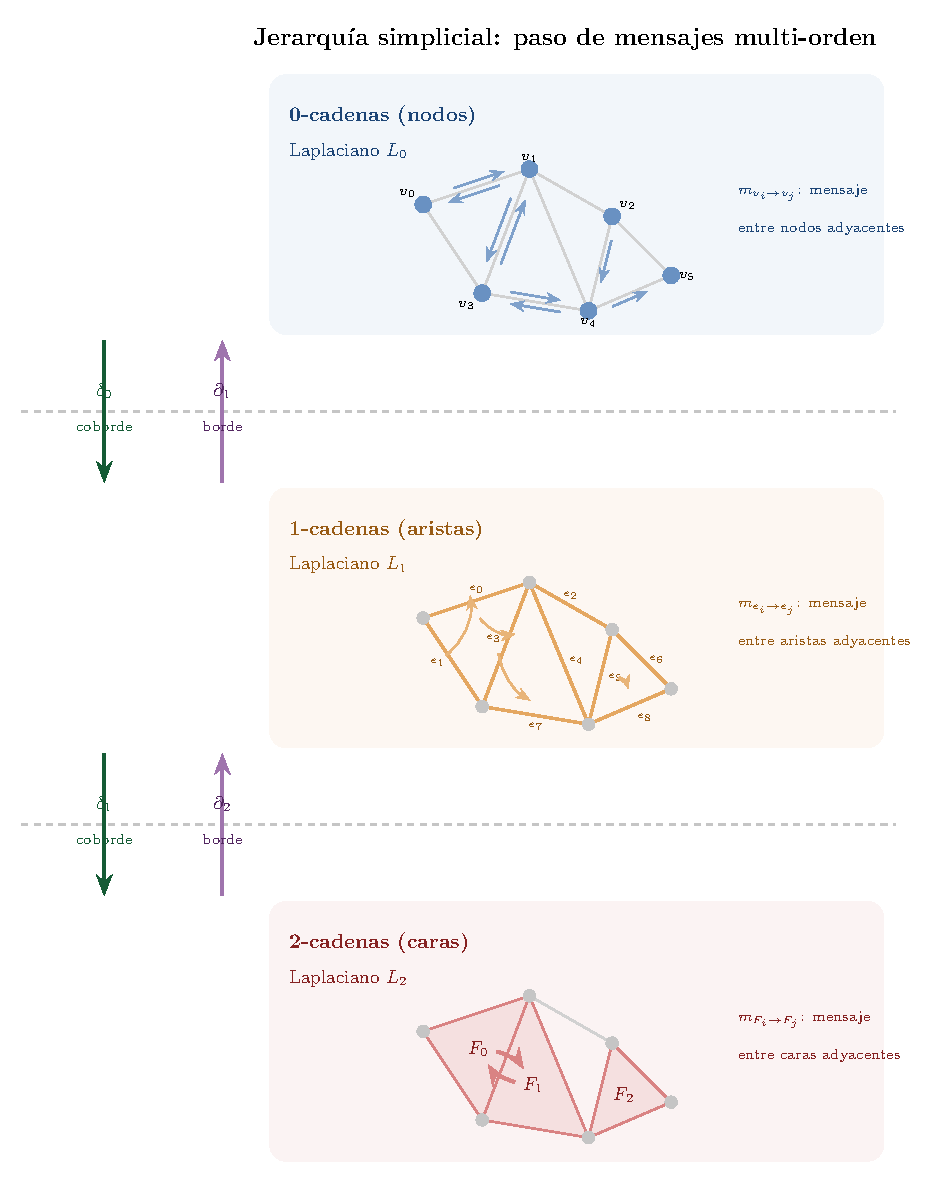
\includegraphics[width=0.85\textwidth]{images/simplicial_hierarchy}
	\caption[Simplicial hierarchy: multi-order message passing]{Message passing hierarchy in a simplicial complex: messages between nodes (0-chains), edges (1-chains) and faces (2-chains), connected by boundary $\partial_k$ and coboundary $\delta_k$ operators. The Hodge Laplacian $L_k$ captures the interaction between adjacent levels.}
	\label{fig:simplicial_hierarchy}
\end{figure}

\subsubsection{Hodge Laplacians}

Hodge Laplacians are fundamental operators that extend the graph Laplacian to higher-dimensional complexes (for the general definition and its properties, see \autoref{def:hodge_laplacian_gdl} and \autoref{prop:propiedades_hodge_gdl} of \autoref{ch:gdl}).

\begin{definition}[Coboundary Operator]\label{def:cofrontera}
The \textbf{coboundary operator} $\delta_k: C_k \to C_{k+1}$ is the formal adjoint of $\partial_{k+1}$:
\[\delta_k = \partial_{k+1}^T\]
with respect to the standard inner product on chain spaces.
\end{definition}

\begin{definition}[Hodge Laplacians]\label{def:hodge_laplacians_cnn}
The \textbf{Hodge Laplacian} of order $k$ is:
\[L_k = \partial_{k+1} \partial_{k+1}^T + \partial_k^T \partial_k = \delta_{k-1} \delta_{k-1}^T + \delta_k^T \delta_k\]

Decomposition into two terms:
\begin{itemize}
    \item $L_k^{\text{down}} = \partial_k^T \partial_k$: Lower Laplacian (flow from $(k-1)$-chains)
    \item $L_k^{\text{up}} = \partial_{k+1} \partial_{k+1}^T$: Upper Laplacian (flow toward $(k+1)$-chains)
\end{itemize}
\end{definition}

\begin{theorem}[Properties of the Hodge Laplacian]\label{thm:prop_hodge_laplacian}
The Laplacian $L_k$ satisfies:
\begin{enumerate}
    \item \textbf{Symmetry}: $L_k$ is symmetric and positive semidefinite
    \item \textbf{Kernel and homology}: $\ker(L_k) \cong H_k(\mathcal{K})$ (homology group of dimension $k$)
    \item \textbf{Hodge decomposition}:
    \[C_k = \text{Im}(\partial_{k+1}) \oplus \ker(L_k) \oplus \text{Im}(\partial_k^T)\]
\end{enumerate}
\end{theorem}

\begin{proof}
(1) \textit{Symmetry}: $L_k = \partial_k^T \partial_k + \partial_{k+1} \partial_{k+1}^T$ is a sum of matrices of the form $A^T A$, which are symmetric and positive semidefinite. To see that $L_k$ is positive semidefinite: $\langle L_k \mathbf{x}, \mathbf{x} \rangle = \|\partial_k \mathbf{x}\|^2 + \|\partial_{k+1}^T \mathbf{x}\|^2 \geq 0$.

(2) \textit{Kernel and homology}: $L_k \mathbf{x} = 0$ if and only if $\|\partial_k \mathbf{x}\|^2 + \|\partial_{k+1}^T \mathbf{x}\|^2 = 0$, that is, $\partial_k \mathbf{x} = 0$ and $\partial_{k+1}^T \mathbf{x} = 0$. The first condition says that $\mathbf{x}$ is a $k$-cycle ($\mathbf{x} \in \ker \partial_k$) and the second that $\mathbf{x}$ is orthogonal to the image of $\partial_{k+1}$ ($\mathbf{x} \perp \operatorname{Im} \partial_{k+1}$). Hence $\ker L_k = \ker \partial_k \cap (\operatorname{Im} \partial_{k+1})^\perp$, which is the harmonic representative of the homology class $H_k = \ker \partial_k / \operatorname{Im} \partial_{k+1}$.

(3) \textit{Hodge decomposition}: The three subspaces are mutually orthogonal: $\operatorname{Im}(\partial_{k+1}) \perp \operatorname{Im}(\partial_k^T)$ because $\partial_k \partial_{k+1} = 0$ (fundamental property of the boundary operators). The kernel $\ker L_k$ is the orthogonal complement of $\operatorname{Im}(\partial_{k+1}) \oplus \operatorname{Im}(\partial_k^T)$ in $C_k$.
\end{proof}

\begin{example}[Hodge Laplacian for a Triangular Mesh]\label{ex:hodge_triangle_mesh}
Consider a simple triangular mesh with 4 vertices forming two adjacent triangles.

\textbf{Structure:}
\begin{itemize}
    \item Vertices: $v_0, v_1, v_2, v_3$
    \item Edges: $e_1 = [v_0,v_1], e_2 = [v_1,v_2], e_3 = [v_0,v_2], e_4 = [v_1,v_3], e_5 = [v_2,v_3]$
    \item Triangles: $\tau_1 = [v_0,v_1,v_2], \tau_2 = [v_1,v_2,v_3]$
\end{itemize}

\textbf{Boundary matrix $\partial_1$ (edges $\to$ vertices):}
\[\partial_1 = \begin{pmatrix}
-1 & 0 & -1 & 0 & 0 \\
1 & -1 & 0 & -1 & 0 \\
0 & 1 & 1 & 0 & -1 \\
0 & 0 & 0 & 1 & 1
\end{pmatrix}\]

\textbf{Boundary matrix $\partial_2$ (triangles $\to$ edges):}

For $\tau_1 = [v_0,v_1,v_2]$: $\partial_2(\tau_1) = [v_1,v_2] - [v_0,v_2] + [v_0,v_1] = e_2 - e_3 + e_1$.
For $\tau_2 = [v_1,v_2,v_3]$: $\partial_2(\tau_2) = [v_2,v_3] - [v_1,v_3] + [v_1,v_2] = e_5 - e_4 + e_2$.
\[\partial_2 = \begin{pmatrix}
1 & 0 \\
1 & 1 \\
-1 & 0 \\
0 & -1 \\
0 & 1
\end{pmatrix}\]

It is verified that $\partial_1 \partial_2 = 0$, consistent with \autoref{thm:partial_squared}.

\textbf{Edge Laplacian (1-Laplacian):}
\[L_1 = \partial_1^T \partial_1 + \partial_2 \partial_2^T\]

This operator captures both the connectivity between edges via common vertices and via common triangles.
\end{example}

\subsubsection{Topological Deep Learning: Architectures}

The comprehensive work of \citet{hajij2023topological} establishes the theoretical and practical foundations of topological deep learning.

\begin{definition}[Combinatorial Complex]\label{def:complejo_combinatorial}
A \textbf{combinatorial complex} $\mathcal{K}$ is a collection of finite sets (cells) equipped with a partial inclusion relation, which generalizes both simplicial and cell complexes without imposing restrictive boundary conditions.
\end{definition}

This definition generalizes traditional relational data structures:
\begin{itemize}
    \item \textbf{Graphs:} Special case with cells of dimension 0 and 1
    \item \textbf{Hypergraphs:} Subset with hyperedges of variable dimension
    \item \textbf{Simplicial complexes:} Restricted case with specific boundary relations
    \item \textbf{Cell complexes:} Generalizations with cells of arbitrary shapes
\end{itemize}

\textbf{Combinatorial Complex Neural Networks (CCNNs):}

CCNNs operate by means of multi-level message passing between cells of different dimensions:
\[h_\sigma^{(l+1)} = \text{UPDATE}\left(h_\sigma^{(l)}, \text{AGGREGATE}\left(\{h_\tau^{(l)} : \tau \in \mathcal{N}(\sigma)\}\right)\right)\]
where $\mathcal{N}(\sigma)$ represents the neighborhood of the cell $\sigma$, which may include cells of various dimensions.

\begin{definition}[Neighborhoods in Complexes]\label{def:vecindarios_complejos}
For a $k$-cell $\sigma$ in a complex, we define:
\begin{itemize}
    \item \textbf{Lower neighborhood}: $\mathcal{N}_{\text{low}}(\sigma) = \{\tau : \tau \subseteq \sigma, \dim(\tau) = k-1\}$
    \item \textbf{Upper neighborhood}: $\mathcal{N}_{\text{up}}(\sigma) = \{\tau : \sigma \subseteq \tau, \dim(\tau) = k+1\}$
    \item \textbf{Co-dimensional neighborhood}: $\mathcal{N}_{\text{co}}(\sigma) = \{\tau : \dim(\tau) = k, \tau \cap \sigma \neq \emptyset\}$
\end{itemize}
\end{definition}

\textbf{Boundary and Co-boundary Operators:}

The topological structure is captured by means of linear operators derived from the algebraic boundary operators:
\begin{itemize}
    \item \textbf{Boundary operator} $\partial_k: C_k \to C_{k-1}$ (see \autoref{def:cadenas_frontera})
    \item \textbf{Co-boundary operator} $\delta_k = \partial_{k+1}^T: C_k \to C_{k+1}$
\end{itemize}

These operators define the generalized adjacency matrices that govern the message passing.

\textbf{Equivariance Properties:}

CCNNs maintain equivariance under:
\begin{enumerate}
    \item \textbf{Permutations}: Reordering of cells within the same dimension
    \item \textbf{Orientations}: Changes in the orientation of oriented cells
    \item \textbf{Topological transformations}: Homeomorphisms that preserve the structure
\end{enumerate}

\subsubsection{Simplicial Attention Networks}

The work of \citet{giusti2022simplicial} introduces attention mechanisms specifically designed for simplicial complexes, combining topological expressiveness with the flexibility of attention.

\textbf{Simplicial Complexes:}

\begin{definition}[Simplicial Complex]
A \textbf{simplicial complex} $\mathcal{K}$ is a collection of simplices that satisfies:
\begin{enumerate}
    \item If $\sigma \in \mathcal{K}$ and $\tau \subseteq \sigma$, then $\tau \in \mathcal{K}$ (downward closure)
    \item The intersection of two simplices is empty or a common simplex
\end{enumerate}
\end{definition}

\textbf{Simplicial Attention Mechanism:}

For a $k$-simplex $\sigma$ and its neighborhood $N(\sigma)$:
\[\alpha_{\sigma,\tau} = \text{softmax}\left(\text{LeakyReLU}\left(a^T[W_\sigma h_\sigma \| W_\tau h_\tau \| o_{\sigma,\tau}]\right)\right)\]
where:
\begin{itemize}
    \item $h_\sigma, h_\tau$: Representations of simplices
    \item $W_\sigma, W_\tau$: Learnable transformation matrices
    \item $a$: Learnable attention vector
    \item $o_{\sigma,\tau}$: Relative orientation information
\end{itemize}

\textbf{Attention with Orientation (Signed Attention):}

A distinctive feature is the incorporation of orientation information:
\[\alpha'_{\sigma,\tau} = s_{\sigma,\tau} \cdot \alpha_{\sigma,\tau}\]
where $s_{\sigma,\tau} \in \{-1, +1\}$ reflects the relative orientation between simplices.

This oriented attention preserves the cohomological properties of the complex and maintains equivariance under orientation changes:
\[\text{SAT}(\mathcal{O}(X)) = \mathcal{O}(\text{SAT}(X))\]
for an orientation change $\mathcal{O}$.

\textbf{Multi-dimensional Processing:}

SATs process information in multiple dimensions simultaneously:
\begin{itemize}
    \item \textbf{Parallel layers:} Independent processing by dimension
    \item \textbf{Inter-dimensional communication:} Flow of information via boundary operators
    \item \textbf{Hierarchical aggregation:} Topologically-aware pooling
\end{itemize}

\subsubsection{CW Complexes and Applications}

CW (Closure-finite, Weak topology) complexes provide an even more general framework than simplicial complexes, allowing cells of arbitrary shapes attached in a topologically coherent way.

\textbf{Definition and Structure:}

\begin{definition}[CW Complex]
A \textbf{CW complex} is a topological space $X$ together with a decomposition into cells $e^n_\alpha$ of dimension $n$, where each cell is attached to the lower-dimensional skeleton by means of a continuous characteristic map.
\end{definition}

\textbf{Advantages for Deep Learning:}
\begin{enumerate}
    \item \textbf{Geometric flexibility:} Cells of arbitrary shapes
    \item \textbf{Representational efficiency:} Fewer cells than equivalent simplicial representations
    \item \textbf{Computational compatibility:} Regular structure compatible with parallelization
\end{enumerate}

\textbf{Emerging Applications:}
\begin{itemize}
    \item \textbf{Image analysis:} Segmentation based on topological structure
    \item \textbf{Molecular modeling:} Representation of protein complexes
    \item \textbf{Neuroscience:} Analysis of brain connectomes
    \item \textbf{Social network analysis:} Modeling of hierarchical communities
\end{itemize}

\subsection{Connections between Algebra and Topology}

The true power of advanced algebraic extensions emerges from the deep connections between algebraic and topological structures. These connections are not merely theoretical, but provide unifying principles for the design of \gls{GDL} architectures.

\subsubsection{Homology and Cohomology}

Homology and cohomology provide algebraic invariants of topological spaces that are fundamental to \gls{GDL}.

We recall that the $k$-th homology group $H_k(\mathcal{K}) = Z_k / B_k$ measures the ``$k$-dimensional holes'' of the complex (\autoref{def:homologia_betti} of \autoref{ch:gdl}).\label{def:grupos_homologia_cnn}

\textbf{Geometric Interpretation.}\label{rem:interp_homologia} $H_k(\mathcal{K})$ measures the ``$k$-dimensional holes'' of the space:
\begin{itemize}
    \item $H_0$: Connected components
    \item $H_1$: Non-trivial cycles (tunnels, loops)
    \item $H_2$: Cavities (voids)
    \item $H_k$ ($k > 2$): Higher-dimensional holes
\end{itemize}

\begin{definition}[Betti Numbers]\label{def:numeros_betti_cnn}
The \textbf{$k$-th Betti number} is:
\[\beta_k = \dim(H_k(\mathcal{K})) = \text{rank}(Z_k) - \text{rank}(B_k)\]
\end{definition}

\begin{example}[Homology of the Sphere and Torus]\label{ex:homologia_esfera_toro}
\textbf{Sphere $S^2$:}
\begin{align}
H_0(S^2) &\cong \mathbb{R} \quad (\beta_0 = 1, \text{ connected}) \\
H_1(S^2) &= 0 \quad (\beta_1 = 0, \text{ no loops}) \\
H_2(S^2) &\cong \mathbb{R} \quad (\beta_2 = 1, \text{ cavity})
\end{align}

\textbf{Torus $T^2 = S^1 \times S^1$:}
\begin{align}
H_0(T^2) &\cong \mathbb{R} \quad (\beta_0 = 1) \\
H_1(T^2) &\cong \mathbb{R}^2 \quad (\beta_1 = 2, \text{ two independent loops}) \\
H_2(T^2) &\cong \mathbb{R} \quad (\beta_2 = 1)
\end{align}

The Euler characteristic:
\[\chi(S^2) = \beta_0 - \beta_1 + \beta_2 = 1 - 0 + 1 = 2\]
\[\chi(T^2) = \beta_0 - \beta_1 + \beta_2 = 1 - 2 + 1 = 0\]
\end{example}

\begin{definition}[De Rham Cohomology]\label{def:cohomologia_derham}
On differentiable manifolds, the \textbf{De Rham cohomology} $H^k_{\text{dR}}(\mathcal{M})$ is defined as:
\[H^k_{\text{dR}}(\mathcal{M}) = \frac{\ker(d: \Omega^k \to \Omega^{k+1})}{\text{Im}(d: \Omega^{k-1} \to \Omega^k)}\]
where $\Omega^k$ is the space of differential $k$-forms and $d$ is the exterior derivative.
\end{definition}

\begin{theorem}[De Rham Theorem]\label{thm:derham}
For a differentiable manifold $\mathcal{M}$:
\[H^k_{\text{dR}}(\mathcal{M}) \cong H^k(\mathcal{M}; \mathbb{R})\]
The De Rham cohomology is isomorphic to the singular cohomology with real coefficients.

See Section~\ref{sec:de_rham} of \autoref{ch:teoremas_complementarios} for the proof.
\end{theorem}

\subsubsection{Exterior Algebra and Connection with Clifford}

The exterior algebra provides the bridge between Clifford algebras and algebraic topology.

\begin{definition}[Exterior Algebra]\label{def:algebra_exterior}
Let $V$ be a vector space. The \textbf{exterior algebra} $\bigwedge V$ is the graded algebra:
\[\bigwedge V = \bigoplus_{k=0}^n \bigwedge^k V\]
where $\bigwedge^k V$ is the space of $k$-vectors with antisymmetric exterior product $\wedge$:
\[v \wedge w = -w \wedge v, \quad v \wedge v = 0\]
\end{definition}

\textbf{Clifford-Exterior Relation.}\label{rem:clifford_exterior} The Clifford algebra $\text{Cl}(V, Q)$ and the exterior algebra $\bigwedge V$ are related:
\begin{itemize}
    \item As vector spaces: $\text{Cl}(V,Q) \cong \bigwedge V$ (both have dimension $2^n$)
    \item The geometric product extends the exterior product: $uv = u \cdot v + u \wedge v$
    \item $\bigwedge V = \text{Cl}(V, 0)$ (Clifford algebra with null quadratic form)
\end{itemize}

\begin{example}[Basis of the Exterior Algebra $\bigwedge \mathbb{R}^3$]\label{ex:base_exterior_3d}
For $V = \mathbb{R}^3$ with basis $\{e_1, e_2, e_3\}$:
\begin{align}
\bigwedge^0 \mathbb{R}^3 &: \{1\} \quad \text{(scalars)} \\
\bigwedge^1 \mathbb{R}^3 &: \{e_1, e_2, e_3\} \quad \text{(vectors)} \\
\bigwedge^2 \mathbb{R}^3 &: \{e_1 \wedge e_2, e_1 \wedge e_3, e_2 \wedge e_3\} \quad \text{(bivectors)} \\
\bigwedge^3 \mathbb{R}^3 &: \{e_1 \wedge e_2 \wedge e_3\} \quad \text{(pseudoscalar)}
\end{align}
Total: $1 + 3 + 3 + 1 = 8$ dimensions.
\end{example}

\subsubsection{Persistent Homology}

Persistent homology provides a multiscale tool for the topological analysis of data.

\begin{definition}[Filtration]\label{def:filtracion_cnn}
A \textbf{filtration} of a simplicial complex is a nested sequence:
\[\emptyset = \mathcal{K}_0 \subseteq \mathcal{K}_1 \subseteq \mathcal{K}_2 \subseteq \cdots \subseteq \mathcal{K}_m = \mathcal{K}\]
where each $\mathcal{K}_i$ is a subcomplex of $\mathcal{K}$.
\end{definition}

\begin{definition}[Persistence Diagram]\label{def:diagrama_persistencia_cnn}
The \textbf{persistence diagram} records the pairs $(b, d)$ where:
\begin{itemize}
    \item $b$ (birth): Scale at which a homological cycle appears
    \item $d$ (death): Scale at which the cycle disappears
    \item Persistence: $\text{pers}(b,d) = d - b$
\end{itemize}
\end{definition}

\textbf{Applications in GDL.}\label{rem:persistencia_gdl} Persistent homology is used in:
\begin{itemize}
    \item \textbf{Featurization}: Persistence diagrams as features for CNNs
    \item \textbf{Topological pooling}: Preserving persistent structures
    \item \textbf{Regularization}: Penalizing undesired topologies
\end{itemize}

\subsubsection{Sheaf Theory}

Sheaf theory provides a framework for data distributed over topological spaces.

\begin{definition}[Cellular Sheaf]\label{def:sheaf_celular}
A \textbf{cellular sheaf} $\mathcal{F}$ over a cell complex $X$ assigns:
\begin{itemize}
    \item To each cell $\sigma \in X$ a vector space $\mathcal{F}(\sigma)$ (stalk)
    \item To each pair $\tau \subseteq \sigma$ a restriction map $\mathcal{F}_{\sigma \to \tau}: \mathcal{F}(\sigma) \to \mathcal{F}(\tau)$
\end{itemize}
satisfying composition properties.
\end{definition}

\textbf{Sheaf Neural Networks.}\label{rem:sheaf_nns} The Sheaf Neural Networks of \citet{hansen2021sheaf} and \citet{bodnar2023cellular} use sheaves to model:
\begin{itemize}
    \item \textbf{Heterogeneity}: Different feature spaces in each cell
    \item \textbf{Alignment}: Restriction maps as alignment transformations
    \item \textbf{Coherence}: Minimizing misalignment in the message passing
\end{itemize}

\begin{example}[Sheaf Laplacian]\label{ex:sheaf_laplacian}
For a sheaf $\mathcal{F}$ over a graph $G$, the \textbf{sheaf Laplacian} is:
\[L_{\mathcal{F}} = \delta^T \delta\]
where $\delta$ incorporates the restriction maps:
\[(\delta f)_e = \mathcal{F}_{t(e) \to e}(f_{t(e)}) - \mathcal{F}_{s(e) \to e}(f_{s(e)})\]
for an edge $e$ with source $s(e)$ and target $t(e)$.

It generalizes the standard graph Laplacian by allowing heterogeneous feature spaces.
\end{example}

\subsubsection{Learnable Topological Invariants}

Advanced architectures can learn to compute topological invariants such as:
\begin{itemize}
    \item \textbf{Betti numbers:} Dimensions of homology groups (\autoref{def:numeros_betti_cnn})
    \item \textbf{Euler characteristic:} Alternating sum of Betti numbers: $\chi = \sum_k (-1)^k \beta_k$
    \item \textbf{Characteristic classes:} Differentiable invariants of bundles
    \item \textbf{Persistence diagrams:} Multiscale representations of topology
\end{itemize}

These invariants provide robust and geometrically meaningful representations for learning.

\subsubsection{Categorical Perspectives}

Category theory provides a unifying language that connects Clifford algebras, topological complexes, and neural network architectures.

\textbf{Functors and Equivalences.}\label{rem:funtores_equivalencias} The functors between geometric categories formalize the transformations of representation:
\begin{itemize}
    \item \textbf{Chains functor}: $C_*: \textbf{Top} \to \textbf{Chain}$ (spaces to chain complexes)
    \item \textbf{Homology functor}: $H_*: \textbf{Chain} \to \textbf{GrVect}$ (chains to graded spaces)
    \item \textbf{Clifford functor}: Associates to each Riemannian manifold its Clifford bundle
\end{itemize}

The advanced algebraic extensions (Clifford, topological, categorical) face computational challenges of scalability and numerical stability in high-dimensional algebras, and require further theoretical development in expressive capabilities and convergence guarantees.

\section{Special Methods and Connections}\label{sec:special_methods}

This final section of the chapter explores specialized methods that complement the geometric convolutional techniques presented earlier, establishing connections with other learning paradigms and analyzing future perspectives of the field. The topics covered include advanced positional encoding, controlled symmetry breaking, applications in quantum computing, and scalability considerations that determine the practical viability of these methods.

\subsection{Positional Encoding and Fourier Features}

\subsubsection{Foundations of Positional Encoding}

Positional encoding represents a fundamental challenge in geometric learning: how to represent spatial information in a way that preserves both the local structure and the global relations. Traditional CNNs incorporate positional information implicitly through the neighborhood structure of convolutions, but in more general geometric contexts this approach proves insufficient.

The seminal work of \citet{tancik2020fourier} demonstrated that standard neural networks have difficulty learning functions that vary rapidly in low-dimensional domains. This problem arises because networks with \gls{ReLU} activations are naturally biased toward smooth functions, a limitation that manifests especially in tasks that require capturing high-frequency details.

\begin{theorem}[Frequency Bias in Neural Networks]
Let $f: \mathbb{R}^d \to \mathbb{R}$ be a target function with significant spectral components at high frequencies. A neural network $\mathcal{F}_\theta$ trained by gradient descent in the parameter space $\theta$ exhibits a bias toward the approximation of low-frequency components of $f$ during the first iterations of training.
\end{theorem}

This bias originates in the weight initialization and the nature of gradient descent, which tends to explore first the components of the function space of lower complexity. Mathematically, consider the Fourier expansion of the target function:
\begin{equation}
f(\mathbf{x}) = \sum_{\omega \in \mathbb{Z}^d} \hat{f}(\omega) e^{2\pi i \omega \cdot \mathbf{x}}
\end{equation}

During the first epochs of training, the network preferentially approximates the coefficients $\hat{f}(\omega)$ with small $\|\omega\|$, postponing the capture of high-frequency components.

\subsubsection{Random Fourier Features: Foundational Theory}

The pioneering work of Rahimi \& Recht (NIPS 2007) established the theoretical foundations of random Fourier features for approximating kernels in large-scale kernel machines. This approach has become a fundamental tool for positional encoding in geometric learning.

\begin{theorem}[Bochner's Theorem]\label{thm:bochner}
A continuous kernel $k: \mathbb{R}^d \times \mathbb{R}^d \to \mathbb{R}$ is translation invariant (i.e., $k(\mathbf{x}, \mathbf{y}) = k(\mathbf{x} - \mathbf{y})$) and positive definite if and only if there exists a finite non-negative probability measure $\mu$ such that:
\begin{equation}
k(\mathbf{x} - \mathbf{y}) = \int_{\mathbb{R}^d} e^{2\pi i \omega^T (\mathbf{x} - \mathbf{y})} d\mu(\omega)
\end{equation}
\end{theorem}

\begin{proof}
The forward direction follows from basic properties of the Fourier transform. For the reverse direction, the function $\phi(\mathbf{x}) = k(\mathbf{x}, \mathbf{0}) = k(\mathbf{x})$ is continuous and positive definite. By the classical Bochner theorem, $\phi$ admits a representation as the Fourier transform of a finite non-negative measure.
\end{proof}

Bochner's theorem provides the mathematical justification for approximating kernels by Monte Carlo sampling of their Fourier transform. If $p(\omega)$ is the density associated with $\mu$, we can approximate:
\begin{equation}
k(\mathbf{x}, \mathbf{y}) \approx \frac{1}{m} \sum_{j=1}^m \cos(2\pi \omega_j^T \mathbf{x}) \cos(2\pi \omega_j^T \mathbf{y}) + \sin(2\pi \omega_j^T \mathbf{x}) \sin(2\pi \omega_j^T \mathbf{y})
\end{equation}
where $\omega_j \sim p(\omega)$ are independently sampled frequencies.

\paragraph{Construction of the Feature Mapping}

We define the random Fourier features mapping as:
\begin{equation}
z(\mathbf{x}) = \sqrt{\frac{2}{m}} \begin{bmatrix} \cos(2\pi \omega_1^T \mathbf{x}) \\ \vdots \\ \cos(2\pi \omega_m^T \mathbf{x}) \\ \sin(2\pi \omega_1^T \mathbf{x}) \\ \vdots \\ \sin(2\pi \omega_m^T \mathbf{x}) \end{bmatrix} \in \mathbb{R}^{2m}
\end{equation}

This mapping satisfies the fundamental property:
\begin{equation}
\mathbb{E}_{\omega \sim p}[z(\mathbf{x})^T z(\mathbf{y})] = k(\mathbf{x}, \mathbf{y})
\end{equation}

\begin{theorem}[Convergence of Random Fourier Features]
Let $k$ be a Gaussian kernel $k(\mathbf{x}, \mathbf{y}) = \exp(-\|\mathbf{x} - \mathbf{y}\|^2 / 2\sigma^2)$ and $\hat{k}_m$ its approximation by $m$ random Fourier features. Then, for any $\epsilon, \delta > 0$, if:
\begin{equation}
m \geq \frac{4}{\epsilon^2} \log\left(\frac{2n}{\delta}\right)
\end{equation}
it holds that with probability at least $1 - \delta$:
\begin{equation}
\sup_{\mathbf{x}, \mathbf{y} \in \mathcal{X}} |k(\mathbf{x}, \mathbf{y}) - \hat{k}_m(\mathbf{x}, \mathbf{y})| \leq \epsilon
\end{equation}
where $\mathcal{X} \subset \mathbb{R}^d$ is a compact set of $n$ points.

See Section~\ref{sec:convergencia_rff} of \autoref{ch:teoremas_complementarios} for the complete proof.
\end{theorem}

This result guarantees uniform convergence of the approximation with rate $O(1/\sqrt{m})$, providing rigorous theoretical guarantees for the use of random Fourier features in positional encoding.

\subsubsection{Fourier Features as Universal Encoding}

The solution proposed by Tancik et al. consists of transforming the input coordinates by means of Fourier features before processing them with the neural network. For an input $\mathbf{x} \in \mathbb{R}^d$, the Fourier features transformation is defined as:

\begin{equation}
\gamma(\mathbf{x}) = \left[\sin(2\pi \mathbf{B}\mathbf{x}), \cos(2\pi \mathbf{B}\mathbf{x})\right]^T
\end{equation}

where $\mathbf{B} \in \mathbb{R}^{m \times d}$ is a frequency matrix sampled from a Gaussian distribution $\mathcal{N}(0, \sigma^2)$. The parameter $\sigma$ controls the frequency spectrum: small values favor smooth functions while large values allow high-frequency variations to be captured.

\begin{definition}[Fourier Features Mapping]
A Fourier features mapping $\gamma: \mathbb{R}^d \to \mathbb{R}^{2m}$ is a transformation that projects spatial coordinates to a feature space where periodic functions of different frequencies can be represented linearly.
\end{definition}

\paragraph{Spectral Analysis and Choice of $\sigma$}

The choice of the scale parameter $\sigma$ in the frequency distribution is crucial. For Gaussian RBF kernels $k(\mathbf{x}, \mathbf{y}) = \exp(-\|\mathbf{x} - \mathbf{y}\|^2 / 2\gamma^2)$, the optimal frequency distribution is $p(\omega) \propto \exp(-\|\omega\|^2 \gamma^2 / 2)$, that is, $\omega \sim \mathcal{N}(0, \gamma^{-2} \mathbf{I})$.

In practice, $\sigma$ is selected by cross-validation or following heuristics based on the characteristic scale of the data:
\begin{equation}
\sigma_{\text{optimal}} \approx \frac{1}{\text{median}(\{\|\mathbf{x}_i - \mathbf{x}_j\| : i, j \in [n]\})}
\end{equation}

\paragraph{Worked Example: Encoding in $\mathbb{R}^2$}

Consider spatial coordinates $\mathbf{x} = (x, y) \in [0, 1]^2$ and $m = 3$ frequency components. We sample:
\begin{align}
\omega_1 &= (2.1, -1.3)^T, \quad \omega_2 = (-0.8, 3.4)^T, \quad \omega_3 = (1.7, 2.2)^T
\end{align}

The Fourier encoding for a point $\mathbf{x}_0 = (0.5, 0.5)$ is:
\begin{align}
\gamma(\mathbf{x}_0) = [&\sin(2\pi \cdot 0.4), \sin(2\pi \cdot 1.3), \sin(2\pi \cdot 1.95), \\
&\cos(2\pi \cdot 0.4), \cos(2\pi \cdot 1.3), \cos(2\pi \cdot 1.95)]^T
\end{align}

This encoding captures information about the position at multiple frequency scales simultaneously.

\subsubsection{Connection with Harmonic Analysis on Manifolds}

This technique has profound implications for geometric CNNs. On Riemannian manifolds, the geodesic coordinates can be enriched with Fourier features to capture high-frequency local variations while preserving the global structure of the manifold.

Harmonic analysis on manifolds provides the theoretical framework for extending random Fourier features to non-Euclidean domains. Let $(\mathcal{M}, g)$ be a compact Riemannian manifold with Laplace-Beltrami operator $\Delta_{\mathcal{M}}$. The eigenfunctions $\{\phi_k\}$ of the Laplacian form a complete orthonormal basis of $L^2(\mathcal{M})$:
\begin{equation}
\Delta_{\mathcal{M}} \phi_k = -\lambda_k \phi_k, \quad \int_{\mathcal{M}} \phi_i \phi_j \, dV_g = \delta_{ij}
\end{equation}

\begin{proposition}[Fourier Features on Manifolds]
For a compact Riemannian manifold $\mathcal{M}$, a feature mapping based on eigenfunctions of the Laplacian:
\begin{equation}
\gamma_{\mathcal{M}}(p) = \sqrt{\frac{2}{m}} \begin{bmatrix} \phi_1(p) \\ \vdots \\ \phi_m(p) \end{bmatrix}
\end{equation}
approximates diffusion kernels $k_t(p, q) = \sum_{k=1}^\infty e^{-t\lambda_k} \phi_k(p)\phi_k(q)$ with error $O(e^{-t\lambda_{m+1}})$.
\end{proposition}

\begin{proof}
The diffusion kernel expands as $k_t(p,q) = \sum_{k=1}^{\infty} e^{-t\lambda_k} \phi_k(p) \phi_k(q)$, where $\{\lambda_k, \phi_k\}$ are the eigenpairs of the Laplace-Beltrami operator on $\mathcal{M}$ with $0 \leq \lambda_1 \leq \lambda_2 \leq \cdots$. The approximation with $m$ eigenfunctions truncates the series: $\hat{k}_t(p,q) = \sum_{k=1}^{m} e^{-t\lambda_k} \phi_k(p) \phi_k(q)$. The truncation error is:
\[
|k_t(p,q) - \hat{k}_t(p,q)| = \left|\sum_{k=m+1}^{\infty} e^{-t\lambda_k} \phi_k(p) \phi_k(q)\right| \leq e^{-t\lambda_{m+1}} \sum_{k=m+1}^{\infty} |\phi_k(p) \phi_k(q)|
\]
where we used $e^{-t\lambda_k} \leq e^{-t\lambda_{m+1}}$ for $k > m$. The convergence of the residual series is guaranteed by Weyl's law ($\lambda_k \sim k^{2/\dim \mathcal{M}}$) and the uniform bound on the eigenfunctions on compact manifolds.
\end{proof}

This result establishes that the eigenfunctions of the Laplacian on manifolds generalize the sinusoidal functions of the Euclidean case, providing a unified theory of positional encoding.

\subsubsection{Integration with Equivariant CNNs}

The combination of Fourier features with equivariant CNNs requires special care to preserve the symmetry properties. Let $g \in G$ be a transformation of the symmetry group and $\mathbf{x}$ a spatial coordinate. For the encoding to be equivariant, it must satisfy:

\begin{equation}
\gamma(g \cdot \mathbf{x}) = \rho(g) \gamma(\mathbf{x})
\end{equation}

where $\rho: G \to \text{GL}(\mathbb{R}^{2m})$ is a representation of the group in the feature space.

For rotation groups $\text{SO}(2)$, this is achieved using circular harmonics as a basis for the Fourier features. Specifically, for $G = \text{SO}(2)$, the frequencies $\omega$ must be selected so that $\omega \cdot (R\mathbf{x}) = (R^T\omega) \cdot \mathbf{x}$ for every rotation $R \in \text{SO}(2)$.

For rotations in 3D ($G = \text{SO}(3)$), the spherical harmonics $Y_\ell^m(\theta, \phi)$ provide the natural equivariant basis. The encoding is constructed as:
\begin{equation}
\gamma_{\text{SO}(3)}(\mathbf{x}) = [Y_0^0(\theta, \phi), Y_1^{-1}(\theta, \phi), Y_1^0(\theta, \phi), Y_1^1(\theta, \phi), \ldots]^T
\end{equation}
where $(\theta, \phi)$ are spherical coordinates associated with $\mathbf{x}$.

\paragraph{Equivariance for the Euclidean Group $E(3)$}

For the full Euclidean group $E(3) = \mathbb{R}^3 \rtimes \text{SO}(3)$ (rotations and translations), the construction is more complex. Features are used that separate magnitude information (invariant to rotations) and direction (equivariant):
\begin{equation}
\gamma_{E(3)}(\mathbf{x}) = [\|\mathbf{x}\|, Y_\ell^m(\hat{\mathbf{x}})]
\end{equation}
where $\hat{\mathbf{x}} = \mathbf{x}/\|\mathbf{x}\|$ is the unit direction.

\subsubsection{Applications in Differential Geometry}

In the context of manifolds, Fourier features can be adapted to respect the local Riemannian metric. Given a coordinate atlas $\{(U_i, \phi_i)\}$ for a manifold $\mathcal{M}$, the features are constructed as:

\begin{equation}
\gamma_{\mathcal{M}}(p) = \gamma(\phi_i(p)) \sqrt{|\det(g_{ij}(p))|}
\end{equation}

where $g_{ij}$ is the metric tensor in local coordinates. This modification ensures that the features are invariant under coordinate changes and reflect the intrinsic geometry of the manifold.

\paragraph{Gauge Theory and Fourier Features}

In principal bundles, Fourier features can incorporate gauge connection information. Let $(P, \mathcal{M}, \pi, G)$ be a principal bundle with connection $\omega$. The gauge-equivariant positional encoding is defined by means of:
\begin{equation}
\gamma_{\text{gauge}}(p) = \Gamma_\gamma^{-1} \gamma(\pi(p))
\end{equation}
where $\Gamma_\gamma$ is the parallel transport along a curve $\gamma$ from a base point to $\pi(p)$.

This construction guarantees that the features transform appropriately under local gauge transformations, preserving the geometric structure of the bundle.

\subsection{Controlled Symmetry Breaking}

\subsubsection{Theoretical Motivation}

Although equivariance is desirable for the generalization and data efficiency of models, in many real applications the symmetries are approximate or there is privileged information that breaks the natural symmetries. The work of \citet{vanderouderaa2024symmetry} formalizes the concept of controlled symmetry breaking as a regularization technique that allows models to adapt to deviations from perfect symmetry.

\begin{definition}[Controlled Symmetry Breaking]
A controlled symmetry breaking is an intentional modification of an equivariant architecture that introduces a specific directional bias while maintaining the ability to revert to equivariant behavior when the data require it.
\end{definition}

The mathematical formulation is based on the interpolation between equivariant and invariant operators. Let $\mathcal{F}_{\text{eq}}: X \to Y$ be an equivariant function and $\mathcal{F}_{\text{in}}: X \to Y$ an invariant function. The function with controlled breaking is defined as:

\begin{equation}
\mathcal{F}_\lambda = (1-\lambda) \mathcal{F}_{\text{eq}} + \lambda \mathcal{F}_{\text{in}}
\end{equation}

where $\lambda \in [0,1]$ is a parameter that controls the degree of symmetry breaking.

\paragraph{Group Theory Foundations}

To formalize controlled breaking mathematically, let $G$ be a group of symmetries acting on the input space $X$ and $\rho: G \to \text{GL}(Y)$ a representation in the output space. A function $f: X \to Y$ is $G$-equivariant if:
\begin{equation}
f(g \cdot x) = \rho(g) f(x), \quad \forall g \in G, x \in X
\end{equation}

Symmetry breaking introduces a parametrized family $f_\lambda$ that interpolates between full equivariance ($\lambda = 0$) and symmetry independence ($\lambda = 1$):
\begin{equation}
f_\lambda(g \cdot x) = (1-\lambda) \rho(g) f_\lambda(x) + \lambda h(g \cdot x)
\end{equation}
where $h: X \to Y$ is an auxiliary function without equivariance constraints.

\begin{proposition}[Smoothness of the Transition]
The family $\{f_\lambda\}_{\lambda \in [0,1]}$ defines a continuous curve in the function space. If $f_0$ is $G$-equivariant and $h$ is arbitrary, then:
\begin{equation}
\lim_{\lambda \to 0} \|f_\lambda(g \cdot x) - \rho(g) f_\lambda(x)\| = 0
\end{equation}
uniformly over compacts in $X \times G$.
\end{proposition}

\begin{proof}
Let $f_\lambda = (1-\lambda) f_0 + \lambda h$ with $f_0$ equivariant and $h$ arbitrary. For $g \in G$:
\begin{align}
\|f_\lambda(g \cdot x) - \rho(g) f_\lambda(x)\| &= \|(1-\lambda)(f_0(g \cdot x) - \rho(g) f_0(x)) + \lambda(h(g \cdot x) - \rho(g) h(x))\| \\
&= \lambda \|h(g \cdot x) - \rho(g) h(x)\|
\end{align}
where we used the exact equivariance of $f_0$. Over a compact $K \subset X \times G$, the continuous function $(x,g) \mapsto \|h(g \cdot x) - \rho(g) h(x)\|$ is bounded by some $M < \infty$. Thus, $\|f_\lambda(g \cdot x) - \rho(g) f_\lambda(x)\| \leq \lambda M \to 0$ as $\lambda \to 0$, uniformly over $K$.
\end{proof}

\subsubsection{Implementation in Geometric CNNs}

In the context of CNNs on manifolds, symmetry breaking can be implemented in several ways:

\textbf{1. Breaking in the Feature Space:} A directional bias is introduced in the intermediate representations:

\begin{equation}
\mathbf{h}_{l+1} = \sigma(\mathbf{W}_l * \mathbf{h}_l + \mathbf{b}_l + \lambda_l \mathbf{v}_{\text{bias}})
\end{equation}

where $\mathbf{v}_{\text{bias}}$ is a bias vector that breaks the symmetry in a controlled way.

\textbf{2. Breaking in the Convolutions:} The convolutional kernels include asymmetric components:

\begin{equation}
K_{\text{sb}}(\mathbf{x}, \mathbf{y}) = K_{\text{sym}}(\mathbf{x}, \mathbf{y}) + \lambda K_{\text{asym}}(\mathbf{x}, \mathbf{y})
\end{equation}

where $K_{\text{sym}}$ preserves the symmetries of the problem and $K_{\text{asym}}$ introduces a specific directionality.

\textbf{3. Adaptive Breaking:} The parameter $\lambda$ is learned during training, allowing the model to automatically determine the optimal degree of symmetry breaking for each layer or region of the input space.

The loss function for adaptive breaking incorporates a regularization term:
\begin{equation}
\mathcal{L}_{\text{total}} = \mathcal{L}_{\text{task}} + \alpha \sum_{l=1}^L \lambda_l^2
\end{equation}
where $\alpha > 0$ controls the bias toward equivariant solutions.

\paragraph{Variational Formulation}

From a Bayesian perspective, controlled breaking can be formulated as variational inference over the function space. We define a prior distribution $p(\lambda)$ that favors small values of $\lambda$:
\begin{equation}
p(\lambda) = \text{Beta}(\alpha, \beta), \quad \alpha > \beta > 0
\end{equation}

The posterior distribution $p(\lambda | \mathcal{D})$ is inferred from the data by means of:
\begin{equation}
p(\lambda | \mathcal{D}) \propto p(\mathcal{D} | \lambda) p(\lambda)
\end{equation}

This approach allows the uncertainty about the optimal degree of symmetry breaking to be quantified.

\subsubsection{Regularization Analysis}

Controlled symmetry breaking acts as a regularization mechanism that prevents overfitting to perfect symmetries that may not exist in real data. From an information-theoretic perspective, symmetry breaking introduces additional capacity to the model while maintaining an inductive bias toward symmetric solutions.

\begin{theorem}[Regularizing Effect of Symmetry Breaking]
Let $\mathcal{H}_{\text{eq}}$ be the space of equivariant hypotheses and $\mathcal{H}_{\lambda}$ the space with controlled breaking. Then:
\[\text{VC-dim}(\mathcal{H}_{\lambda}) = \text{VC-dim}(\mathcal{H}_{\text{eq}}) + O(\lambda \log(1/\lambda))\]
\end{theorem}

\begin{proof}[Proof sketch]
The Vapnik-Chervonenkis dimension measures the capacity of the hypothesis space. For $\lambda = 0$, we recover $\mathcal{H}_{\text{eq}}$. As $\lambda$ increases, additional directions are added in the function space. The logarithmic growth derives from the analysis of the covering of orbits under the action of $G$.
\end{proof}

This result shows that controlled breaking expands the capacity of the model logarithmically in the breaking parameter, providing additional flexibility without drastically compromising the generalization capacity.

\paragraph{Bias-Variance Trade-off}

Symmetry breaking modifies the classical bias-variance trade-off of statistical learning. For an estimator $\hat{f}_\lambda$ with symmetry breaking $\lambda$, the expected error decomposes as:
\begin{align}
\mathbb{E}[\|f - \hat{f}_\lambda\|^2] &= \underbrace{\|f - \mathbb{E}[\hat{f}_\lambda]\|^2}_{\text{Bias}^2} + \underbrace{\mathbb{E}[\|\hat{f}_\lambda - \mathbb{E}[\hat{f}_\lambda]\|^2]}_{\text{Variance}} \\
&= B(\lambda)^2 + V(\lambda)
\end{align}

where typically $B(\lambda)$ decreases and $V(\lambda)$ increases with $\lambda$, suggesting the existence of an optimal value $\lambda^*$.

\subsubsection{Practical Applications}

\paragraph{Natural Images with Directional Biases}

In photography, although objects can have intrinsic symmetry, factors such as directional lighting and gravity break the symmetry systematically. A CNN with controlled breaking can capture these effects:
\begin{equation}
\mathbf{h}^{(l)} = \text{ReLU}(W_{\text{eq}}^{(l)} * \mathbf{h}^{(l-1)} + \lambda_l \mathbf{b}_{\text{gravity}})
\end{equation}
where $\mathbf{b}_{\text{gravity}}$ encodes a vertical bias consistent with gravity.

\paragraph{Molecular Data with Approximate Symmetries}

In computational chemistry, molecules can have nominal symmetries that are broken by environmental or quantum effects. GNNs with controlled breaking model these deviations:
\begin{equation}
\mathbf{h}_v^{(l+1)} = \sum_{u \in \mathcal{N}(v)} [(1-\lambda) \phi_{\text{eq}}(\mathbf{h}_u^{(l)}, \mathbf{e}_{vu}) + \lambda \phi_{\text{asym}}(\mathbf{h}_u^{(l)}, \mathbf{e}_{vu}, \mathbf{c}_{\text{env}})]
\end{equation}
where $\mathbf{c}_{\text{env}}$ encodes environmental conditions that break the symmetry.

\subsection{Connections with Quantum Computing}

\subsubsection{Equivariant Quantum CNNs}

The intersection between geometric deep learning and quantum computing represents an emerging frontier with transformative potential. The work of \citet{west2024quantum} explores how the principles of equivariance extend naturally to the quantum regime, where quantum states and unitary operations respect fundamental symmetries of physics.

An equivariant quantum CNN operates in the Hilbert space $\mathcal{H} = (\mathbb{C}^2)^{\otimes n}$, where the quantum states $|\psi\rangle$ encode geometric information. Equivariance manifests through commutation with quantum symmetry operators:

\begin{equation}
[U_g, \mathcal{C}_\text{quantum}] = 0
\end{equation}

where $U_g$ is the unitary representation of the group element $g$ and $\mathcal{C}_\text{quantum}$ is the quantum convolutional operation.

\subsubsection{Embedding of Geometric Data}

The embedding of classical data in quantum states requires specialized techniques that preserve the geometric structure. For data on manifolds, the embedding is performed by means of:

\begin{equation}
|\psi(\mathbf{x})\rangle = \sum_{i=1}^{2^n} \alpha_i(\mathbf{x}) |i\rangle
\end{equation}

where the amplitudes $\alpha_i(\mathbf{x})$ encode the local coordinates in the manifold so that the geometric symmetries translate into symmetries of the quantum state.

\textbf{Fundamental Advantages of the Quantum Approach:}

\begin{itemize}
\item \textbf{Coherent Superposition:} The superposition principle allows the simultaneous evaluation of geometric configurations in the Hilbert space $\mathcal{H} = \bigotimes_{i=1}^n \mathbb{C}^{d_i}$.
\item \textbf{Geometric Entanglement:} Entangled states $|\psi\rangle \in \mathcal{H}_A \otimes \mathcal{H}_B$ naturally encode non-separable correlations between geometrically distant regions.
\item \textbf{Exponential Encoding:} The dimension of the Hilbert space grows exponentially, allowing dense representations of complex geometric structures using $\log_2(\dim \mathcal{H})$ qubits.
\end{itemize}

\subsubsection{Measurement and Decoherence}

The measurement process in quantum CNNs must be designed carefully to extract relevant geometric information while minimizing the loss of quantum coherence. Projective measurements are used in bases that respect the symmetries of the problem:

\begin{equation}
P_{\text{sym}} = \frac{1}{|G|} \sum_{g \in G} U_g P_0 U_g^\dagger
\end{equation}

where $P_0$ is a base projector and the sum over the group $G$ ensures that the measurement is invariant under the relevant symmetries.

\subsection{Scalability and Efficiency Analysis}

\subsubsection{The Equivariance vs. Scalability Dilemma}

A fundamental theoretical result established by \citet{park2024equivariancescale} examines the saturation of the advantages of equivariance in high-dimensionality regimes. This analysis reveals an intrinsic tension between geometric constraints and expressive capacity in hypothesis spaces of great complexity.

\begin{hypothesis}[Equivariance Saturation Hypothesis]
There exists a scale regime where the benefits of equivariance saturate and the additional capacity of the model can compensate for the loss of geometric inductive bias.
\end{hypothesis}

This saturation has theoretical foundations based on universal approximation theory and the Vapnik-Chervonenkis dimension:

\begin{itemize}
\item The symmetry orbits in high-dimensional spaces require exponential coverage
\item The Rademacher complexity of equivariant functions is related to the size of the group
\item There is a fundamental trade-off between expressive capacity and geometric constraints
\end{itemize}

\paragraph{Quantitative Analysis of Orbit Coverage}

For a finite group $G$ acting on $\mathbb{R}^d$, the number of distinct orbits in a ball of radius $R$ grows as:
\begin{equation}
|\{\text{Orbits in } B_R\}| \sim \frac{\text{Vol}(B_R)}{|G| \cdot \text{Vol}(\text{fundamental domain})}
\end{equation}

In high dimensions ($d \to \infty$), the volume $\text{Vol}(B_R) = \frac{\pi^{d/2}}{\Gamma(d/2 + 1)} R^d$ grows exponentially, requiring an exponential number of parameters to cover all orbits with fixed resolution.

\begin{proposition}[Parametric Cost of Equivariance]
Let $\mathcal{F}_{\text{eq}}$ be a family of $G$-equivariant functions and $\mathcal{F}_{\text{free}}$ functions without constraints. To achieve approximation error $\epsilon$ over a compact domain, the number of required parameters satisfies:
\begin{equation}
\frac{N_{\text{eq}}}{N_{\text{free}}} \geq \left(\frac{|G|}{\text{const}}\right)^{1/d}
\end{equation}
in the high-dimensional limit.
\end{proposition}

\begin{proof}[Proof sketch]
A $G$-equivariant function $f: \mathbb{R}^d \to \mathbb{R}^d$ satisfies $f(gx) = gf(x)$ for all $g \in G$, which imposes $|G|$ constraints for each point of the domain. These constraints reduce the effective degrees of freedom by a factor $|G|$, so that the space $\mathcal{F}_{\text{eq}}$ has dimension $\sim N/|G|$ per unit of volume of the domain. However, to \textit{approximate} arbitrary functions (not necessarily equivariant), an equivariant network needs to compensate for the imposed constraints. In high dimension $d$, the ``curse of dimensionality'' implies that the number of parameters needed to cover the compact domain grows exponentially in $d$, and the reduction by symmetry is attenuated as $(|G|/\text{const})^{1/d}$ by the packing properties in high dimension.
\end{proof}

This result suggests that in sufficiently high dimensions, equivariant architectures require significantly more parameters to achieve the same expressive capacity.

\subsubsection{Computational Complexity: Big-O Analysis}

We analyze the temporal and spatial complexity of different geometric architectures.

\paragraph{Graph Convolutional Networks (GCN)}

For a graph with $|V| = n$ vertices and $|E| = m$ edges:

\textbf{Temporal Complexity:}
\begin{itemize}
\item A GCN layer: $O(m \cdot d_{\text{in}} \cdot d_{\text{out}})$
\item Complete network ($L$ layers): $O(L \cdot m \cdot d^2)$ where $d = \max(d_{\text{in}}, d_{\text{out}})$
\end{itemize}

\textbf{Spatial Complexity:}
\begin{itemize}
\item Storage of representations: $O(L \cdot n \cdot d)$
\item Adjacency matrix (dense): $O(n^2)$
\item Adjacency matrix (sparse): $O(m)$
\end{itemize}

\paragraph{Graph Attention Networks (GAT)}

\textbf{Temporal Complexity:}
\begin{itemize}
\item Attention computation: $O(m \cdot d + n \cdot h \cdot d^2)$ where $h$ is the number of heads
\item Multi-head with $h$ heads: $O(h \cdot m \cdot d + n \cdot h \cdot d^2)$
\item Complete network: $O(L \cdot h \cdot m \cdot d^2)$
\end{itemize}

\textbf{Spatial Complexity:}
\begin{itemize}
\item Attention matrices: $O(h \cdot m)$
\item Cache of intermediate scores: $O(h \cdot n \cdot d)$
\end{itemize}

\paragraph{GraphGPS (Graph GPS Transformer)}

GraphGPS combines local \gls{MPNN} with global attention:

\textbf{Temporal Complexity:}
\begin{itemize}
\item Local \gls{MPNN}: $O(m \cdot d^2)$
\item Global attention: $O(n^2 \cdot d)$ (complete) or $O(n \cdot k \cdot d)$ (approximate with $k$ neighbors)
\item Spectral positional encoding: $O(n^3)$ (precomputation) or $O(n \cdot \log n \cdot d)$ (approximation)
\item Total per layer: $O(m \cdot d^2 + n \cdot k \cdot d + n \cdot \log n \cdot d)$
\end{itemize}

\textbf{Spatial Complexity:}
\begin{itemize}
\item Positional features: $O(n \cdot d_{\text{pos}})$
\item Attention: $O(n \cdot k)$ (approximate) or $O(n^2)$ (complete)
\end{itemize}

\subsubsection{Comparative Table of Architectures}

\begin{table}[h]
\centering
\begin{tabular}{l|c|c|c|c}
\toprule
\textbf{Architecture} & \textbf{Time/layer} & \textbf{Space} & \textbf{Expressiveness} & \textbf{Equivariance} \\
\midrule
GCN & $O(m \cdot d^2)$ & $O(n \cdot d)$ & Medium & Permutation \\
GAT & $O(h \cdot m \cdot d^2)$ & $O(h \cdot m)$ & High & Permutation \\
GraphGPS & $O(n^2 \cdot d)$ & $O(n^2)$ & Very high & Permutation \\
G-CNN & $O(|G| \cdot n \cdot d^2)$ & $O(|G| \cdot n \cdot d)$ & High & $G$-equivariant \\
Steerable CNN & $O(n \cdot d^2 \cdot r^3)$ & $O(n \cdot d)$ & High & SO(3) \\
\bottomrule
\end{tabular}
\caption[Computational complexity of geometric architectures]{Comparison of computational complexity and properties of different geometric architectures. Here $n$ = number of nodes, $m$ = number of edges, $d$ = feature dimension, $h$ = number of heads, $|G|$ = order of the group, $r$ = angular resolution.}
\label{tab:complejidad_arquitecturas_geometricas}
\end{table}

\subsubsection{Metrics of Geometric Efficiency}\label{subsubsec:metricas_eficiencia_geometrica}

To quantify the efficiency of geometric CNNs, the following metrics are proposed:

\textbf{1. Parametric Compression Index:}
\begin{equation}
\text{PCI} = \frac{\dim(\mathcal{H}_{\text{free}})}{\dim(\mathcal{H}_{G\text{-eq}})}
\end{equation}
where $\mathcal{H}_{\text{free}}$ and $\mathcal{H}_{G\text{-eq}}$ are the free and $G$-equivariant hypothesis spaces respectively.

For finite groups, $\text{PCI} = |G|$ approximately. For continuous groups such as $\text{SO}(3)$, the compression depends on the parametrization:
\begin{equation}
\text{PCI}_{\text{SO}(3)} \approx \frac{(2\ell_{\max} + 1)^2}{2\ell_{\max} + 1} = 2\ell_{\max} + 1
\end{equation}
where $\ell_{\max}$ is the maximum degree of spherical harmonics used.

\textbf{2. Geometric Generalization Gain:}
\begin{equation}
\text{GGG} = \frac{\mathcal{R}_{\text{emp}}[\mathcal{H}_{\text{free}}] - \mathcal{R}_{\text{emp}}[\mathcal{H}_{G\text{-eq}}]}{\sqrt{\frac{\log |G|}{n}}}
\end{equation}
where $\mathcal{R}_{\text{emp}}$ is the empirical risk and $n$ the sample size.

This metric normalizes the improvement in generalization by the size of the group and the sample size, providing a fair measure of the geometric benefit.

\textbf{3. Relative Algorithmic Complexity:}
\begin{equation}
\text{RAC} = \frac{\mathcal{C}(\mathcal{A}_{G\text{-eq}})}{\mathcal{C}(\mathcal{A}_{\text{standard}}) \cdot \mathcal{T}(\epsilon)}
\end{equation}
where $\mathcal{C}(\mathcal{A})$ is the algorithmic complexity of the method $\mathcal{A}$ and $\mathcal{T}(\epsilon)$ represents the convergence speedup factor to precision $\epsilon$.

\paragraph{Quantitative Example: Point Cloud Classification}

For the ModelNet40 dataset with $n = 10{,}000$ points per cloud:

\begin{itemize}
\item \textbf{PointNet (baseline)}:
  \begin{itemize}
  \item Complexity: $O(n \cdot d^2)$
  \item PCI: $1$ (no equivariance)
  \item Accuracy: $89.2\%$
  \end{itemize}

\item \textbf{PointNet++ with SO(3) equivariance}:
  \begin{itemize}
  \item Complexity: $O(n \cdot d^2 \cdot (2\ell_{\max} + 1)^2)$ with $\ell_{\max} = 2$
  \item PCI: $5$
  \item Accuracy: $93.7\%$ ($+4.5\%$)
  \item GGG: $\frac{4.5}{\sqrt{\log(5) / 10000}} \approx 352.6$
  \end{itemize}
\end{itemize}

This demonstrates that the generalization gain (GGG) is substantial, justifying the additional cost of equivariance.

\subsubsection{Efficient Scaling Strategies}

To address the scalability challenges, several strategies have been developed:

\textbf{1. Hierarchical Equivariance:} We define a sequence of groups $G_1 \supset G_2 \supset \cdots \supset G_L$ where each layer $l$ maintains $G_l$-equivariance, allowing controlled relaxation of constraints.

\textbf{Example:} In image processing:
\begin{itemize}
\item Early layers: $G_1 = p4m$ (symmetries of the full square)
\item Intermediate layers: $G_2 = p4$ (only $90^\circ$ rotations)
\item Final layers: $G_3 = \{e\}$ (no equivariance)
\end{itemize}

\textbf{2. $\epsilon$-Approximate Equivariance:} For $\epsilon > 0$, a function $f$ is $\epsilon$-equivariant if:
\begin{equation}
\sup_{g \in G} \|f(g \cdot x) - \rho(g)f(x)\| \leq \epsilon
\end{equation}

This provides theoretical flexibility with approximation guarantees. In practice, it is implemented by means of:
\begin{equation}
f_\epsilon(x) = \frac{1}{|S|} \sum_{g \in S} \rho(g)^{-1} f_{\text{approx}}(g \cdot x)
\end{equation}
where $S \subset G$ is a finite subset and $f_{\text{approx}}$ is not exactly equivariant.

\begin{proposition}[Error of $\epsilon$-Equivariance]
If $f_{\text{approx}}$ is $\epsilon$-equivariant and $|S| \geq \log(1/\delta) / \epsilon^2$, then with probability $1 - \delta$:
\begin{equation}
\|f_\epsilon(g \cdot x) - \rho(g) f_\epsilon(x)\| \leq 2\epsilon
\end{equation}
\end{proposition}

\begin{proof}
Let $f_\epsilon$ be an $\epsilon$-equivariant function, that is, $\|f_\epsilon(g \cdot x) - \rho(g) f_\epsilon(x)\| \leq \epsilon$ for all $g \in G$ and $x$ in the domain. Let $S = \{x_1, \ldots, x_{|S|}\}$ be a set of i.i.d. samples from the domain. By the triangle inequality, for any $g \in G$ and $x$ in the domain:
\[
\|f_\epsilon(g \cdot x) - \rho(g) f_\epsilon(x)\| \leq \|f_\epsilon(g \cdot x) - f_\epsilon(g \cdot x_i)\| + \|f_\epsilon(g \cdot x_i) - \rho(g) f_\epsilon(x_i)\| + \|\rho(g)(f_\epsilon(x_i) - f_\epsilon(x))\|
\]
where $x_i$ is the sample closest to $x$. The second term is bounded by $\epsilon$. For $|S| \geq \log(1/\delta)/\epsilon^2$, the concentration of measure guarantees that the discretization error (first and third terms) contributes at most an additional $\epsilon$ with probability $1 - \delta$, giving the total bound $2\epsilon$.
\end{proof}

\textbf{3. Measurable Conditional Equivariance:} It is defined by means of a measurable selection function $\chi: X \to \{0,1\}$ such that:
\begin{equation}
f(g \cdot x) = \chi(x) \rho(g)f(x) + (1-\chi(x))h(g \cdot x)
\end{equation}
where $h$ has no equivariance constraints.

The function $\chi$ is learned jointly with the model parameters, allowing the model to dynamically decide when to apply equivariance constraints.

\textbf{4. Low-Rank Approximation Techniques:}

To reduce the attention complexity in GraphGPS, low-rank factorizations are used:
\begin{equation}
\mathbf{A} = \mathbf{U} \mathbf{V}^T, \quad \mathbf{U}, \mathbf{V} \in \mathbb{R}^{n \times r}, \quad r \ll n
\end{equation}

This reduces the complexity from $O(n^2 \cdot d)$ to $O(n \cdot r \cdot d)$ with controlled error:
\begin{equation}
\|\mathbf{A} - \mathbf{U}\mathbf{V}^T\|_F \leq \sqrt{\sum_{i=r+1}^n \sigma_i^2}
\end{equation}
where $\sigma_i$ are singular values of $\mathbf{A}$.

\paragraph{Algorithmic Optimization: Case Study}

Consider the optimization of an equivariant attention layer in $\text{SO}(3)$:

\textbf{Naive Approach:}
\begin{itemize}
\item Discretize $\text{SO}(3)$ with $N_{\text{rot}}$ rotations
\item Complexity: $O(N_{\text{rot}} \cdot n^2 \cdot d)$
\item For $N_{\text{rot}} = 72$ ($5^\circ$ resolution): $\sim 10^6$ operations per point
\end{itemize}

\textbf{Optimized Approach (spherical harmonics):}
\begin{itemize}
\item Use spherical harmonics of degree $\leq \ell_{\max}$
\item Complexity: $O(n^2 \cdot d \cdot \ell_{\max}^2)$
\item For $\ell_{\max} = 3$: $\sim 10^4$ operations per point
\item \textbf{Speedup}: $100\times$
\end{itemize}

This example illustrates how the mathematical theory (representation theory) leads directly to efficient algorithms.

\subsection{Unifying Synthesis and Future Perspectives}

\subsubsection{Unified Theoretical Framework}

The methods presented in this chapter can be unified under a general theoretical framework that combines:

\begin{itemize}
\item \textbf{Algebraic Structure:} Symmetry groups, Lie algebras, and representations
\item \textbf{Differential Geometry:} Manifolds, connections, and parallel transport
\item \textbf{Harmonic Analysis:} Fourier transforms, spherical harmonics, and wavelets
\item \textbf{Approximation Theory:} Representation capacity and convergence
\end{itemize}

\begin{definition}[Unified Geometric CNN]
A unified geometric CNN is a triple $(\mathcal{M}, G, \Phi)$ where:
\begin{itemize}
\item $\mathcal{M}$ is a Riemannian manifold (possibly with group structure)
\item $G$ is a group of symmetries that acts on $\mathcal{M}$
\item $\Phi$ is a family of equivariant differential operators that generalize the convolution
\end{itemize}
\end{definition}

\subsubsection{Future Research Directions}

\textbf{1. Geometric Approximation Theory:} Development of universal approximation theorems for CNNs on non-compact manifolds and spaces with singularities.

\textbf{2. Optimization on Manifolds:} Optimization algorithms that respect the geometry of the parameter space, especially for models with equivariance constraints.

\textbf{3. Symmetry Learning:} Methods that can automatically discover the relevant symmetries in the data without prior knowledge.

\textbf{4. Quantum Scalability:} Development of quantum CNNs that can process large-scale classical data while maintaining quantum advantage.

\textbf{5. Scientific Applications:} Extension of geometric methods to problems in physics, chemistry, and molecular biology where symmetries are fundamental.

\subsubsection{Connection with Geometric Attention Models}

The developments presented in this chapter establish essential foundations that connect directly with the geometric attention mechanisms explored in \autoref{ch:attention}. This connection is not accidental but reflects a deep convergence in the paradigm of Geometric Deep Learning.

\paragraph{Conceptual Convergence CNN-Attention}

The fundamental concepts developed in the preceding sections find direct parallels in geometric attention:

\begin{itemize}
\item \textbf{\gls{equivarianza} (Section~\ref{subsec:equivarianza_invarianza})}: The equivariant attention mechanisms of \autoref{ch:attention} extend the equivariance constraints of CNNs by means of adaptive weights that respect symmetries.

\item \textbf{\gls{analisis_armonico} (\autoref{sec:analisis_armonico})}: The spectral techniques developed here provide the mathematical basis for the spectral positional encoding in Graph Attention Networks (\autoref{sec:graph_attention}).

\item \textbf{Group convolutions (\autoref{sec:group_convolutions})}: G-CNNs anticipate the formulation of attention over homogeneous spaces.

\item \textbf{Gauge equivariance (\autoref{sec:gauge_cnns})}: The principal bundles introduced here reappear in Geometric Algebra Transformers (\autoref{sec:clifford_attention}), where gauge transformations are realized by means of geometric products and Clifford operations.
\end{itemize}

\paragraph{Unifying Framework: Geometric Message Passing}

Geometric CNNs can be reinterpreted as special cases of the \gls{marco_unificador} of message passing that is formalized completely in \autoref{ch:attention}:

\begin{definition}[CNN as Structured Message Passing]\label{def:cnn_as_structured_mp}
A geometric CNN over domain $\mathcal{D}$ with symmetry group $G$ is a Message Passing Neural Network where:
\begin{itemize}
    \item The underlying graph reflects the geometric structure of $\mathcal{D}$
    \item The message functions preserve the equivariance to $G$
    \item The aggregation respects the local geometry (convolution → locally weighted sum)
    \item The weights are shared according to the orbits of $G$
\end{itemize}
\end{definition}

This perspective, developed completely in \autoref{subsubsec:unified_framework_advanced}, shows how the structural rigidity of CNNs generalizes toward the adaptive flexibility of attention.

\paragraph{Limitations that Motivate Attention}

The limitations identified in traditional CNNs (Section~\ref{subsec:fundamentos_limitaciones_cnn}) directly motivate the developments of \autoref{ch:attention}:

\begin{itemize}
\item \textbf{Long-range dependencies}: The inherent locality of convolutions (limited receptive field) is overcome by means of global attention mechanisms while preserving equivariance. Graph Transformers and Geometric Transformers implement global attention over graphs and manifolds respectively, allowing arbitrarily distant dependencies to be captured without sacrificing geometric properties.

\item \textbf{Irregular geometries}: Complex manifolds with variable curvature and non-trivial topology require adaptive attention patterns that generalize the fixed convolutional kernels. In \autoref{ch:attention}, attention kernels are developed that adapt to the local curvature by means of parallel transport and Riemannian metrics.

\item \textbf{Dimensionality and scalability}: Attention-based methods allow the treatment of high-dimensional spaces by means of low-rank approximation techniques and matrix factorizations, as analyzed in §\ref{subsubsec:metricas_eficiencia_geometrica}. These techniques are implemented in Linformer, Performer, and Flash Attention, demonstrating that scalability does not require sacrificing geometric expressiveness.

\item \textbf{Data heterogeneity}: CNNs assume homogeneous data in regular domains. Attention mechanisms, especially in Graph Attention Networks and Heterogeneous Graph Transformers, naturally handle heterogeneous data with multiple types of nodes and edges, each with its own feature space and symmetries.
\end{itemize}

\paragraph{Theoretical Bridge: From Convolution to Attention}

The mathematical transition from convolution to attention can be formalized by means of:

\begin{theorem}[Attention as Generalization of Convolution]
A geometric convolution operation $f * g$ on a manifold $\mathcal{M}$ can be expressed as a limit case of attention:
\begin{equation}
(f * g)(x) = \lim_{\beta \to \infty} \int_{\mathcal{M}} \frac{e^{-\beta d(x,y)^2}}{\int_{\mathcal{M}'} e^{-\beta d(x,y')^2} dy'} g(y) f(y) \, dy
\end{equation}
where $d$ is the Riemannian distance and the limit $\beta \to \infty$ recovers locally compact support.
\end{theorem}

\begin{proof}[Proof sketch]
The Gaussian kernel $K_\beta(x,y) = e^{-\beta d(x,y)^2}$ defines a family of distributions parametrized by $\beta > 0$. For $\beta \to \infty$, $K_\beta(x,y) \to 0$ exponentially fast for all $y \neq x$, while $K_\beta(x,x) = 1$. The normalized distribution $\frac{K_\beta(x,y)}{\int K_\beta(x,y') dy'}$ converges weakly to the Dirac delta $\delta_x(y)$, recovering the locality of the convolution. For finite $\beta$, the attention weights distribute mass in a geodesic neighborhood of radius $\sim 1/\sqrt{\beta}$, producing a ``smoothed'' convolution whose support narrows with $\beta$. See \autoref{ch:attention} for the complete proof.
\end{proof}

This result, proved formally in \autoref{ch:attention}, establishes that attention with Gaussian kernel $K(x,y) = \exp(-\beta d(x,y)^2)$ interpolates continuously between global attention ($\beta \to 0$) and local convolution ($\beta \to \infty$).

\subsubsection{Interdisciplinary Connections}

The field of geometric deep learning is evolving toward a truly interdisciplinary discipline that connects:

\begin{itemize}
\item \textbf{Mathematics:} Differential geometry, representation theory, harmonic analysis, algebraic topology
\item \textbf{Theoretical Physics:} Conformal field theory, gauge theory, geometry of curved spacetimes
\item \textbf{Applied Mathematics:} Approximation theory, functional analysis, dynamical systems
\item \textbf{Logic and Foundations:} Category theory, homological algebra, non-commutative geometry
\end{itemize}

The convergence of these fields suggests that geometric deep learning is not simply a computational tool, but a unifying mathematical language for the extraction of structure from complex data.
